\appendix

\section{Additional Robustness Assets}

This appendix is reserved for supplementary tables and figures that may be moved out of the main text during a later submission-preparation pass. Candidate appendix materials include full weight-sensitivity grids, execution-capacity stress tests, Pareto summaries, Favorita sample-size robustness outputs, Walmart stress-window outputs, Walmart weekly-cadence outputs, and additional Rossmann robustness experiments if those analyses are completed.

\subsection{Walmart Supplementary Robustness Assets}

The Walmart supplementary assets report holiday and markdown stress windows, weekly cadence constraints, and the full Walmart robustness summary. These tables are included for review and should not be interpreted as final conclusions before the result patterns are audited.

\begin{table}
\centering
\caption{Walmart holiday and markdown-heavy stress-window summary.}
\label{tab:walmart-holiday-markdown-stress-by-window}
\resizebox{\textwidth}{!}{%
\begin{tabular}{llllllllllllrrrrrrrrrrrrrrrrrl}
\toprule
dataset\_name & run\_mode &           feature\_set &          experiment\_name &          window\_type & scenario\_name &                   method\_name &  deployable &                oracle\_type &  fallback\_used & fallback\_type & fallback\_reason &  WAPE &  inventory\_cost &  planning\_volatility &  execution\_penalty &  execution\_violation\_rate &  model\_switch\_count &  max\_period\_plan\_change\_pct &  normalized\_inventory\_component &  normalized\_volatility\_component &  normalized\_execution\_component &  normalized\_switch\_component &  normalized\_total\_loss &  gap\_to\_dp\_oracle &  gap\_to\_perfect\_oracle &  rank\_by\_WAPE &  rank\_by\_execution\_penalty &  rank\_by\_normalized\_total\_loss &                          strategy \\
\midrule
     walmart &    quick &          history\_only &  holiday\_markdown\_stress &               normal &      baseline &  Realized-Inventory Oracle DP &       False &  realized\_inventory\_oracle &          False &          none &            none & 0.038 &     7882543.969 &              100.331 &          11347.603 &                     0.017 &                1309 &                       1.949 &                           0.600 &                            0.107 &                           0.017 &                        0.328 &                  1.052 &             0.000 &                 -0.101 &             2 &                          1 &                              1 &    oracle\_dp\_feasibility\_selector \\
     walmart &    quick &          history\_only &  holiday\_markdown\_stress &               normal &      baseline &        Realized Demand Oracle &       False &      perfect\_demand\_oracle &          False &          none &            none & 0.000 &     4115833.731 &              194.115 &         422645.826 &                     0.123 &                   0 &                       5.459 &                           0.313 &                            0.207 &                           0.632 &                        0.000 &                  1.152 &             0.101 &                  0.000 &             1 &                          8 &                              2 &            oracle\_realized\_demand \\
     walmart &    quick &          history\_only &  holiday\_markdown\_stress &               normal &      baseline &                   Budgeted DP &        True &                       none &          False &          none &            none & 0.058 &    13550293.578 &               76.851 &          32374.772 &                     0.011 &                 102 &                       4.143 &                           1.031 &                            0.082 &                           0.048 &                        0.026 &                  1.187 &             0.135 &                  0.035 &             5 &                          4 &                              3 &  budgeted\_dp\_feasibility\_selector \\
     walmart &    quick &          history\_only &  holiday\_markdown\_stress &               normal &      baseline &                   Global Best &        True &                       none &          False &          none &            none & 0.057 &    13141862.485 &               93.868 &          66845.875 &                     0.036 &                   0 &                       3.912 &                           1.000 &                            0.100 &                           0.100 &                        0.000 &                  1.200 &             0.148 &                  0.048 &             3 &                          7 &                              4 &                 global\_best\_model \\
     walmart &    quick &          history\_only &  holiday\_markdown\_stress &               normal &      baseline &                DP Feasibility &        True &                       none &          False &          none &            none & 0.057 &    13405197.135 &               77.169 &          32123.493 &                     0.009 &                 213 &                       4.143 &                           1.020 &                            0.082 &                           0.048 &                        0.053 &                  1.204 &             0.152 &                  0.051 &             4 &                          3 &                              5 &           dp\_feasibility\_selector \\
     walmart &    quick &          history\_only &  holiday\_markdown\_stress &               normal &      baseline &          Operational Ensemble &        True &                       none &          False &          none &            none & 0.061 &    14722668.539 &               69.087 &          30977.986 &                     0.021 &                   0 &                       3.119 &                           1.120 &                            0.074 &                           0.046 &                        0.000 &                  1.240 &             0.188 &                  0.088 &             8 &                          2 &                              6 &         operational\_loss\_ensemble \\
     walmart &    quick &          history\_only &  holiday\_markdown\_stress &               normal &      baseline &               Simple Ensemble &        True &                       none &          False &          none &            none & 0.060 &    14487117.040 &               81.613 &          35526.693 &                     0.026 &                   0 &                       3.439 &                           1.102 &                            0.087 &                           0.053 &                        0.000 &                  1.242 &             0.191 &                  0.090 &             7 &                          6 &                              7 &                   simple\_ensemble \\
     walmart &    quick &          history\_only &  holiday\_markdown\_stress &               normal &      baseline &            Greedy Feasibility &        True &                       none &          False &          none &            none & 0.059 &    14063617.514 &               83.588 &          34606.282 &                     0.013 &                 186 &                       4.143 &                           1.070 &                            0.089 &                           0.052 &                        0.047 &                  1.258 &             0.206 &                  0.105 &             6 &                          5 &                              8 &       greedy\_feasibility\_selector \\
     walmart &    quick &          history\_only &  holiday\_markdown\_stress &              holiday &      baseline &                   Budgeted DP &        True &                       none &          False &          none &            none & 0.071 &     2526532.541 &                9.084 &            165.498 &                     0.005 &                   9 &                       1.542 &                           1.049 &                            0.109 &                           0.003 &                        0.026 &                  1.186 &            -0.046 &                 -2.988 &             5 &                          2 &                              1 &  budgeted\_dp\_feasibility\_selector \\
     walmart &    quick &          history\_only &  holiday\_markdown\_stress &              holiday &      baseline &                   Global Best &        True &                       none &          False &          none &            none & 0.069 &     2409172.941 &                8.350 &           5554.443 &                     0.015 &                   0 &                       0.596 &                           1.000 &                            0.100 &                           0.100 &                        0.000 &                  1.200 &            -0.032 &                 -2.974 &             3 &                          7 &                              2 &                 global\_best\_model \\
     walmart &    quick &          history\_only &  holiday\_markdown\_stress &              holiday &      baseline &            Greedy Feasibility &        True &                       none &          False &          none &            none & 0.071 &     2544462.226 &                9.379 &            165.498 &                     0.005 &                  16 &                       1.542 &                           1.056 &                            0.112 &                           0.003 &                        0.046 &                  1.217 &            -0.015 &                 -2.957 &             6 &                          2 &                              3 &       greedy\_feasibility\_selector \\
     walmart &    quick &          history\_only &  holiday\_markdown\_stress &              holiday &      baseline &                DP Feasibility &        True &                       none &          False &          none &            none & 0.071 &     2538515.091 &                8.972 &            165.498 &                     0.005 &                  19 &                       1.542 &                           1.054 &                            0.107 &                           0.003 &                        0.054 &                  1.218 &            -0.014 &                 -2.955 &             4 &                          2 &                              4 &           dp\_feasibility\_selector \\
     walmart &    quick &          history\_only &  holiday\_markdown\_stress &              holiday &      baseline &  Realized-Inventory Oracle DP &       False &  realized\_inventory\_oracle &          False &          none &            none & 0.049 &     1498825.205 &               12.500 &              6.693 &                     0.015 &                 161 &                       0.305 &                           0.622 &                            0.150 &                           0.000 &                        0.460 &                  1.232 &             0.000 &                 -2.942 &             2 &                          1 &                              5 &    oracle\_dp\_feasibility\_selector \\
     walmart &    quick &          history\_only &  holiday\_markdown\_stress &              holiday &      baseline &          Operational Ensemble &        True &                       none &          False &          none &            none & 0.075 &     2898220.998 &                6.271 &           3248.052 &                     0.020 &                   0 &                       0.500 &                           1.203 &                            0.075 &                           0.058 &                        0.000 &                  1.337 &             0.105 &                 -2.837 &             7 &                          5 &                              6 &         operational\_loss\_ensemble \\
     walmart &    quick &          history\_only &  holiday\_markdown\_stress &              holiday &      baseline &               Simple Ensemble &        True &                       none &          False &          none &            none & 0.076 &     2913711.016 &                7.524 &           3985.786 &                     0.020 &                   0 &                       0.571 &                           1.209 &                            0.090 &                           0.072 &                        0.000 &                  1.371 &             0.139 &                 -2.802 &             8 &                          6 &                              7 &                   simple\_ensemble \\
     walmart &    quick &          history\_only &  holiday\_markdown\_stress &              holiday &      baseline &        Realized Demand Oracle &       False &      perfect\_demand\_oracle &          False &          none &            none & 0.000 &      471152.918 &               29.455 &         201373.427 &                     0.197 &                   0 &                       2.337 &                           0.196 &                            0.353 &                           3.625 &                        0.000 &                  4.174 &             2.942 &                  0.000 &             1 &                          8 &                              8 &            oracle\_realized\_demand \\
     walmart &    quick &          history\_only &  holiday\_markdown\_stress &       markdown\_heavy &      baseline &  Realized-Inventory Oracle DP &       False &  realized\_inventory\_oracle &          False &          none &            none & 0.034 &     2810027.581 &               22.737 &            769.532 &                     0.006 &                 373 &                       1.363 &                           0.537 &                            0.116 &                           0.010 &                        0.460 &                  1.124 &             0.000 &                 -1.258 &             2 &                          1 &                              1 &    oracle\_dp\_feasibility\_selector \\
     walmart &    quick &          history\_only &  holiday\_markdown\_stress &       markdown\_heavy &      baseline &                   Global Best &        True &                       none &          False &          none &            none & 0.053 &     5230508.992 &               19.574 &           7686.896 &                     0.020 &                   0 &                       1.363 &                           1.000 &                            0.100 &                           0.100 &                        0.000 &                  1.200 &             0.076 &                 -1.181 &             3 &                          6 &                              2 &                 global\_best\_model \\
     walmart &    quick &          history\_only &  holiday\_markdown\_stress &       markdown\_heavy &      baseline &                   Budgeted DP &        True &                       none &          False &          none &            none & 0.054 &     5489217.130 &               22.250 &           1519.096 &                     0.009 &                  21 &                       2.383 &                           1.049 &                            0.114 &                           0.020 &                        0.026 &                  1.209 &             0.085 &                 -1.173 &             5 &                          3 &                              3 &  budgeted\_dp\_feasibility\_selector \\
     walmart &    quick &          history\_only &  holiday\_markdown\_stress &       markdown\_heavy &      baseline &                DP Feasibility &        True &                       none &          False &          none &            none & 0.054 &     5473900.394 &               22.601 &           1519.319 &                     0.011 &                  41 &                       2.383 &                           1.047 &                            0.115 &                           0.020 &                        0.051 &                  1.232 &             0.108 &                 -1.149 &             4 &                          4 &                              4 &           dp\_feasibility\_selector \\
     walmart &    quick &          history\_only &  holiday\_markdown\_stress &       markdown\_heavy &      baseline &            Greedy Feasibility &        True &                       none &          False &          none &            none & 0.055 &     5666680.051 &               23.674 &           1515.175 &                     0.009 &                  40 &                       2.383 &                           1.083 &                            0.121 &                           0.020 &                        0.049 &                  1.273 &             0.150 &                 -1.108 &             7 &                          2 &                              5 &       greedy\_feasibility\_selector \\
     walmart &    quick &          history\_only &  holiday\_markdown\_stress &       markdown\_heavy &      baseline &          Operational Ensemble &        True &                       none &          False &          none &            none & 0.055 &     5902660.054 &               16.391 &           5420.401 &                     0.017 &                   0 &                       1.681 &                           1.129 &                            0.084 &                           0.071 &                        0.000 &                  1.283 &             0.159 &                 -1.099 &             8 &                          5 &                              6 &         operational\_loss\_ensemble \\
     walmart &    quick &          history\_only &  holiday\_markdown\_stress &       markdown\_heavy &      baseline &               Simple Ensemble &        True &                       none &          False &          none &            none & 0.055 &     5813318.384 &               19.620 &           8289.496 &                     0.020 &                   0 &                       1.781 &                           1.111 &                            0.100 &                           0.108 &                        0.000 &                  1.319 &             0.196 &                 -1.062 &             6 &                          7 &                              7 &                   simple\_ensemble \\
     walmart &    quick &          history\_only &  holiday\_markdown\_stress &       markdown\_heavy &      baseline &        Realized Demand Oracle &       False &      perfect\_demand\_oracle &          False &          none &            none & 0.000 &     1703808.794 &               43.839 &         140802.552 &                     0.063 &                   0 &                       2.337 &                           0.326 &                            0.224 &                           1.832 &                        0.000 &                  2.381 &             1.258 &                  0.000 &             1 &                          8 &                              8 &            oracle\_realized\_demand \\
     walmart &    quick &          history\_only &  holiday\_markdown\_stress &  holiday\_or\_markdown &      baseline &  Realized-Inventory Oracle DP &       False &  realized\_inventory\_oracle &          False &          none &            none & 0.037 &     3988637.537 &               33.627 &            776.224 &                     0.009 &                 503 &                       1.363 &                           0.557 &                            0.126 &                           0.006 &                        0.449 &                  1.137 &             0.000 &                 -1.974 &             2 &                          1 &                              1 &    oracle\_dp\_feasibility\_selector \\
     walmart &    quick &          history\_only &  holiday\_markdown\_stress &  holiday\_or\_markdown &      baseline &                   Budgeted DP &        True &                       none &          False &          none &            none & 0.058 &     7495733.405 &               28.828 &           1519.096 &                     0.007 &                  28 &                       2.383 &                           1.046 &                            0.108 &                           0.011 &                        0.025 &                  1.190 &             0.053 &                 -1.921 &             5 &                          3 &                              2 &  budgeted\_dp\_feasibility\_selector \\
     walmart &    quick &          history\_only &  holiday\_markdown\_stress &  holiday\_or\_markdown &      baseline &                   Global Best &        True &                       none &          False &          none &            none & 0.057 &     7166517.663 &               26.749 &          13241.339 &                     0.020 &                   0 &                       1.363 &                           1.000 &                            0.100 &                           0.100 &                        0.000 &                  1.200 &             0.063 &                 -1.912 &             3 &                          7 &                              3 &                 global\_best\_model \\
     walmart &    quick &          history\_only &  holiday\_markdown\_stress &  holiday\_or\_markdown &      baseline &                DP Feasibility &        True &                       none &          False &          none &            none & 0.058 &     7487157.647 &               29.107 &           1519.319 &                     0.009 &                  58 &                       2.383 &                           1.045 &                            0.109 &                           0.011 &                        0.052 &                  1.217 &             0.080 &                 -1.895 &             4 &                          4 &                              4 &           dp\_feasibility\_selector \\
     walmart &    quick &          history\_only &  holiday\_markdown\_stress &  holiday\_or\_markdown &      baseline &            Greedy Feasibility &        True &                       none &          False &          none &            none & 0.059 &     7673529.074 &               30.578 &           1515.175 &                     0.007 &                  54 &                       2.383 &                           1.071 &                            0.114 &                           0.011 &                        0.048 &                  1.245 &             0.107 &                 -1.867 &             6 &                          2 &                              5 &       greedy\_feasibility\_selector \\
     walmart &    quick &          history\_only &  holiday\_markdown\_stress &  holiday\_or\_markdown &      baseline &          Operational Ensemble &        True &                       none &          False &          none &            none & 0.060 &     8270784.503 &               21.488 &           8630.769 &                     0.017 &                   0 &                       1.681 &                           1.154 &                            0.080 &                           0.065 &                        0.000 &                  1.300 &             0.162 &                 -1.812 &             8 &                          5 &                              6 &         operational\_loss\_ensemble \\
     walmart &    quick &          history\_only &  holiday\_markdown\_stress &  holiday\_or\_markdown &      baseline &               Simple Ensemble &        True &                       none &          False &          none &            none & 0.060 &     8179245.384 &               25.645 &          12224.613 &                     0.020 &                   0 &                       1.781 &                           1.141 &                            0.096 &                           0.092 &                        0.000 &                  1.330 &             0.192 &                 -1.782 &             7 &                          6 &                              7 &                   simple\_ensemble \\
     walmart &    quick &          history\_only &  holiday\_markdown\_stress &  holiday\_or\_markdown &      baseline &        Realized Demand Oracle &       False &      perfect\_demand\_oracle &          False &          none &            none & 0.000 &     2088018.438 &               67.527 &         340007.772 &                     0.094 &                   0 &                       2.337 &                           0.291 &                            0.252 &                           2.568 &                        0.000 &                  3.112 &             1.974 &                  0.000 &             1 &                          8 &                              8 &            oracle\_realized\_demand \\
     walmart &    quick &  history\_plus\_context &  holiday\_markdown\_stress &               normal &      baseline &  Realized-Inventory Oracle DP &       False &  realized\_inventory\_oracle &          False &          none &            none & 0.038 &     7886177.095 &               99.713 &          11333.473 &                     0.016 &                1310 &                       1.949 &                           0.598 &                            0.119 &                           0.026 &                        0.376 &                  1.120 &             0.000 &                 -0.384 &             2 &                          1 &                              1 &    oracle\_dp\_feasibility\_selector \\
     walmart &    quick &  history\_plus\_context &  holiday\_markdown\_stress &               normal &      baseline &                   Global Best &        True &                       none &          False &          none &            none & 0.057 &    13187821.306 &               83.513 &          44093.445 &                     0.031 &                   0 &                       3.111 &                           1.000 &                            0.100 &                           0.100 &                        0.000 &                  1.200 &             0.080 &                 -0.303 &             4 &                          7 &                              2 &                 global\_best\_model \\
     walmart &    quick &  history\_plus\_context &  holiday\_markdown\_stress &               normal &      baseline &                   Budgeted DP &        True &                       none &          False &          none &            none & 0.058 &    13459541.162 &               73.973 &          32276.944 &                     0.010 &                  94 &                       4.143 &                           1.021 &                            0.089 &                           0.073 &                        0.027 &                  1.209 &             0.090 &                 -0.294 &             5 &                          4 &                              3 &  budgeted\_dp\_feasibility\_selector \\
     walmart &    quick &  history\_plus\_context &  holiday\_markdown\_stress &               normal &      baseline &                DP Feasibility &        True &                       none &          False &          none &            none & 0.057 &    13343417.020 &               75.320 &          32100.649 &                     0.008 &                 178 &                       4.143 &                           1.012 &                            0.090 &                           0.073 &                        0.051 &                  1.226 &             0.106 &                 -0.277 &             3 &                          3 &                              4 &           dp\_feasibility\_selector \\
     walmart &    quick &  history\_plus\_context &  holiday\_markdown\_stress &               normal &      baseline &            Greedy Feasibility &        True &                       none &          False &          none &            none & 0.058 &    13745633.215 &               81.622 &          34053.652 &                     0.012 &                 170 &                       4.143 &                           1.042 &                            0.098 &                           0.077 &                        0.049 &                  1.266 &             0.147 &                 -0.237 &             6 &                          6 &                              5 &       greedy\_feasibility\_selector \\
     walmart &    quick &  history\_plus\_context &  holiday\_markdown\_stress &               normal &      baseline &          Operational Ensemble &        True &                       none &          False &          none &            none & 0.062 &    14824252.681 &               64.275 &          28925.468 &                     0.018 &                   0 &                       2.856 &                           1.124 &                            0.077 &                           0.066 &                        0.000 &                  1.267 &             0.147 &                 -0.236 &             8 &                          2 &                              6 &         operational\_loss\_ensemble \\
     walmart &    quick &  history\_plus\_context &  holiday\_markdown\_stress &               normal &      baseline &               Simple Ensemble &        True &                       none &          False &          none &            none & 0.060 &    14526906.431 &               79.037 &          33649.601 &                     0.026 &                   0 &                       3.272 &                           1.102 &                            0.095 &                           0.076 &                        0.000 &                  1.272 &             0.153 &                 -0.231 &             7 &                          5 &                              7 &                   simple\_ensemble \\
     walmart &    quick &  history\_plus\_context &  holiday\_markdown\_stress &               normal &      baseline &        Realized Demand Oracle &       False &      perfect\_demand\_oracle &          False &          none &            none & 0.000 &     4115833.731 &              194.115 &         422645.826 &                     0.123 &                   0 &                       5.459 &                           0.312 &                            0.232 &                           0.959 &                        0.000 &                  1.503 &             0.384 &                  0.000 &             1 &                          8 &                              8 &            oracle\_realized\_demand \\
     walmart &    quick &  history\_plus\_context &  holiday\_markdown\_stress &              holiday &      baseline &                   Budgeted DP &        True &                       none &          False &          none &            none & 0.068 &     2381644.177 &                8.621 &            165.498 &                     0.005 &                   7 &                       1.542 &                           1.068 &                            0.106 &                           0.003 &                        0.020 &                  1.196 &            -0.150 &                 -2.862 &             5 &                          1 &                              1 &  budgeted\_dp\_feasibility\_selector \\
     walmart &    quick &  history\_plus\_context &  holiday\_markdown\_stress &              holiday &      baseline &                   Global Best &        True &                       none &          False &          none &            none & 0.067 &     2230000.598 &                8.170 &           5775.458 &                     0.020 &                   0 &                       0.592 &                           1.000 &                            0.100 &                           0.100 &                        0.000 &                  1.200 &            -0.146 &                 -2.859 &             3 &                          7 &                              2 &                 global\_best\_model \\
     walmart &    quick &  history\_plus\_context &  holiday\_markdown\_stress &              holiday &      baseline &            Greedy Feasibility &        True &                       none &          False &          none &            none & 0.068 &     2375248.472 &                9.233 &            165.498 &                     0.005 &                  16 &                       1.542 &                           1.065 &                            0.113 &                           0.003 &                        0.046 &                  1.227 &            -0.120 &                 -2.832 &             4 &                          1 &                              3 &       greedy\_feasibility\_selector \\
     walmart &    quick &  history\_plus\_context &  holiday\_markdown\_stress &              holiday &      baseline &                DP Feasibility &        True &                       none &          False &          none &            none & 0.069 &     2433763.094 &                8.641 &            165.498 &                     0.005 &                  19 &                       1.542 &                           1.091 &                            0.106 &                           0.003 &                        0.054 &                  1.254 &            -0.092 &                 -2.804 &             6 &                          1 &                              4 &           dp\_feasibility\_selector \\
     walmart &    quick &  history\_plus\_context &  holiday\_markdown\_stress &              holiday &      baseline &  Realized-Inventory Oracle DP &       False &  realized\_inventory\_oracle &          False &          none &            none & 0.048 &     1455558.199 &               18.621 &            664.205 &                     0.020 &                 159 &                       5.532 &                           0.653 &                            0.228 &                           0.012 &                        0.454 &                  1.346 &             0.000 &                 -2.712 &             2 &                          4 &                              5 &    oracle\_dp\_feasibility\_selector \\
     walmart &    quick &  history\_plus\_context &  holiday\_markdown\_stress &              holiday &      baseline &          Operational Ensemble &        True &                       none &          False &          none &            none & 0.075 &     2852336.130 &                5.849 &           3151.115 &                     0.015 &                   0 &                       0.493 &                           1.279 &                            0.072 &                           0.055 &                        0.000 &                  1.405 &             0.059 &                 -2.653 &             7 &                          5 &                              6 &         operational\_loss\_ensemble \\
     walmart &    quick &  history\_plus\_context &  holiday\_markdown\_stress &              holiday &      baseline &               Simple Ensemble &        True &                       none &          False &          none &            none & 0.075 &     2881817.402 &                7.018 &           3901.335 &                     0.015 &                   0 &                       0.553 &                           1.292 &                            0.086 &                           0.068 &                        0.000 &                  1.446 &             0.099 &                 -2.613 &             8 &                          6 &                              7 &                   simple\_ensemble \\
     walmart &    quick &  history\_plus\_context &  holiday\_markdown\_stress &              holiday &      baseline &        Realized Demand Oracle &       False &      perfect\_demand\_oracle &          False &          none &            none & 0.000 &      471152.918 &               29.455 &         201373.427 &                     0.197 &                   0 &                       2.337 &                           0.211 &                            0.361 &                           3.487 &                        0.000 &                  4.059 &             2.712 &                  0.000 &             1 &                          8 &                              8 &            oracle\_realized\_demand \\
     walmart &    quick &  history\_plus\_context &  holiday\_markdown\_stress &       markdown\_heavy &      baseline &  Realized-Inventory Oracle DP &       False &  realized\_inventory\_oracle &          False &          none &            none & 0.033 &     2771954.257 &               27.796 &            887.717 &                     0.008 &                 378 &                       5.532 &                           0.540 &                            0.141 &                           0.013 &                        0.455 &                  1.150 &             0.000 &                 -1.447 &             2 &                          1 &                              1 &    oracle\_dp\_feasibility\_selector \\
     walmart &    quick &  history\_plus\_context &  holiday\_markdown\_stress &       markdown\_heavy &      baseline &                   Global Best &        True &                       none &          False &          none &            none & 0.054 &     5131615.701 &               19.689 &           6896.885 &                     0.022 &                   0 &                       1.053 &                           1.000 &                            0.100 &                           0.100 &                        0.000 &                  1.200 &             0.050 &                 -1.396 &             5 &                          6 &                              2 &                 global\_best\_model \\
     walmart &    quick &  history\_plus\_context &  holiday\_markdown\_stress &       markdown\_heavy &      baseline &                   Budgeted DP &        True &                       none &          False &          none &            none & 0.054 &     5417599.275 &               22.228 &           1519.096 &                     0.009 &                  27 &                       2.383 &                           1.056 &                            0.113 &                           0.022 &                        0.033 &                  1.223 &             0.074 &                 -1.373 &             4 &                          3 &                              3 &  budgeted\_dp\_feasibility\_selector \\
     walmart &    quick &  history\_plus\_context &  holiday\_markdown\_stress &       markdown\_heavy &      baseline &                DP Feasibility &        True &                       none &          False &          none &            none & 0.054 &     5366712.339 &               23.039 &           1519.319 &                     0.011 &                  45 &                       2.383 &                           1.046 &                            0.117 &                           0.022 &                        0.054 &                  1.239 &             0.089 &                 -1.357 &             3 &                          4 &                              4 &           dp\_feasibility\_selector \\
     walmart &    quick &  history\_plus\_context &  holiday\_markdown\_stress &       markdown\_heavy &      baseline &            Greedy Feasibility &        True &                       none &          False &          none &            none & 0.055 &     5476698.433 &               23.535 &           1515.175 &                     0.009 &                  38 &                       2.383 &                           1.067 &                            0.120 &                           0.022 &                        0.046 &                  1.255 &             0.105 &                 -1.342 &             7 &                          2 &                              5 &       greedy\_feasibility\_selector \\
     walmart &    quick &  history\_plus\_context &  holiday\_markdown\_stress &       markdown\_heavy &      baseline &          Operational Ensemble &        True &                       none &          False &          none &            none & 0.056 &     5873531.341 &               15.690 &           4936.498 &                     0.023 &                   0 &                       1.031 &                           1.145 &                            0.080 &                           0.072 &                        0.000 &                  1.296 &             0.146 &                 -1.300 &             8 &                          5 &                              6 &         operational\_loss\_ensemble \\
     walmart &    quick &  history\_plus\_context &  holiday\_markdown\_stress &       markdown\_heavy &      baseline &               Simple Ensemble &        True &                       none &          False &          none &            none & 0.055 &     5772229.904 &               19.067 &           8163.536 &                     0.023 &                   0 &                       1.248 &                           1.125 &                            0.097 &                           0.118 &                        0.000 &                  1.340 &             0.190 &                 -1.256 &             6 &                          7 &                              7 &                   simple\_ensemble \\
     walmart &    quick &  history\_plus\_context &  holiday\_markdown\_stress &       markdown\_heavy &      baseline &        Realized Demand Oracle &       False &      perfect\_demand\_oracle &          False &          none &            none & 0.000 &     1703808.794 &               43.839 &         140802.552 &                     0.063 &                   0 &                       2.337 &                           0.332 &                            0.223 &                           2.042 &                        0.000 &                  2.596 &             1.447 &                  0.000 &             1 &                          8 &                              8 &            oracle\_realized\_demand \\
     walmart &    quick &  history\_plus\_context &  holiday\_markdown\_stress &  holiday\_or\_markdown &      baseline &  Realized-Inventory Oracle DP &       False &  realized\_inventory\_oracle &          False &          none &            none & 0.037 &     3936430.047 &               39.330 &            894.409 &                     0.010 &                 507 &                       5.532 &                           0.564 &                            0.150 &                           0.007 &                        0.441 &                  1.162 &             0.000 &                 -2.170 &             2 &                          1 &                              1 &    oracle\_dp\_feasibility\_selector \\
     walmart &    quick &  history\_plus\_context &  holiday\_markdown\_stress &  holiday\_or\_markdown &      baseline &                   Budgeted DP &        True &                       none &          False &          none &            none & 0.058 &     7325834.828 &               28.480 &           1519.096 &                     0.007 &                  34 &                       2.383 &                           1.050 &                            0.108 &                           0.012 &                        0.030 &                  1.200 &             0.038 &                 -2.132 &             4 &                          3 &                              2 &  budgeted\_dp\_feasibility\_selector \\
     walmart &    quick &  history\_plus\_context &  holiday\_markdown\_stress &  holiday\_or\_markdown &      baseline &                   Global Best &        True &                       none &          False &          none &            none & 0.058 &     6979417.984 &               26.304 &          12248.638 &                     0.021 &                   0 &                       1.053 &                           1.000 &                            0.100 &                           0.100 &                        0.000 &                  1.200 &             0.038 &                 -2.132 &             5 &                          7 &                              3 &                 global\_best\_model \\
     walmart &    quick &  history\_plus\_context &  holiday\_markdown\_stress &  holiday\_or\_markdown &      baseline &                DP Feasibility &        True &                       none &          False &          none &            none & 0.057 &     7320432.320 &               29.196 &           1519.319 &                     0.009 &                  63 &                       2.383 &                           1.049 &                            0.111 &                           0.012 &                        0.055 &                  1.227 &             0.065 &                 -2.105 &             3 &                          4 &                              4 &           dp\_feasibility\_selector \\
     walmart &    quick &  history\_plus\_context &  holiday\_markdown\_stress &  holiday\_or\_markdown &      baseline &            Greedy Feasibility &        True &                       none &          False &          none &            none & 0.058 &     7369352.031 &               30.300 &           1515.175 &                     0.007 &                  52 &                       2.383 &                           1.056 &                            0.115 &                           0.012 &                        0.045 &                  1.229 &             0.067 &                 -2.103 &             6 &                          2 &                              5 &       greedy\_feasibility\_selector \\
     walmart &    quick &  history\_plus\_context &  holiday\_markdown\_stress &  holiday\_or\_markdown &      baseline &          Operational Ensemble &        True &                       none &          False &          none &            none & 0.060 &     8222608.763 &               20.628 &           8058.002 &                     0.021 &                   0 &                       1.031 &                           1.178 &                            0.078 &                           0.066 &                        0.000 &                  1.322 &             0.161 &                 -2.009 &             8 &                          5 &                              6 &         operational\_loss\_ensemble \\
     walmart &    quick &  history\_plus\_context &  holiday\_markdown\_stress &  holiday\_or\_markdown &      baseline &               Simple Ensemble &        True &                       none &          False &          none &            none & 0.060 &     8123692.535 &               25.041 &          12064.871 &                     0.022 &                   0 &                       1.248 &                           1.164 &                            0.095 &                           0.098 &                        0.000 &                  1.358 &             0.196 &                 -1.974 &             7 &                          6 &                              7 &                   simple\_ensemble \\
     walmart &    quick &  history\_plus\_context &  holiday\_markdown\_stress &  holiday\_or\_markdown &      baseline &        Realized Demand Oracle &       False &      perfect\_demand\_oracle &          False &          none &            none & 0.000 &     2088018.438 &               67.527 &         340007.772 &                     0.094 &                   0 &                       2.337 &                           0.299 &                            0.257 &                           2.776 &                        0.000 &                  3.332 &             2.170 &                  0.000 &             1 &                          8 &                              8 &            oracle\_realized\_demand \\
\bottomrule
\end{tabular}
}

\end{table}

\begin{table}
\centering
\caption{Walmart weekly cadence constraint summary.}
\label{tab:walmart-weekly-cadence-constraints}
\resizebox{\textwidth}{!}{%
\begin{tabular}{llllllllllllrrrrrrrrrrrrrrrrrl}
\toprule
dataset\_name & run\_mode &           feature\_set &             experiment\_name & window\_type &   scenario\_name &                   method\_name &  deployable &                oracle\_type &  fallback\_used & fallback\_type & fallback\_reason &  WAPE &  inventory\_cost &  planning\_volatility &  execution\_penalty &  execution\_violation\_rate &  model\_switch\_count &  max\_period\_plan\_change\_pct &  normalized\_inventory\_component &  normalized\_volatility\_component &  normalized\_execution\_component &  normalized\_switch\_component &  normalized\_total\_loss &  gap\_to\_dp\_oracle &  gap\_to\_perfect\_oracle &  rank\_by\_WAPE &  rank\_by\_execution\_penalty &  rank\_by\_normalized\_total\_loss &                          strategy \\
\midrule
     walmart &    quick &          history\_only &  weekly\_cadence\_constraints &         all &  weekly\_cadence &  Realized-Inventory Oracle DP &       False &  realized\_inventory\_oracle &          False &          none &            none & 0.038 &    11871181.507 &              133.958 &          12123.827 &                     0.014 &                1812 &                       1.949 &                           0.585 &                            0.111 &                           0.015 &                        0.414 &                  1.124 &             0.000 &                 -0.350 &             2 &                          1 &                              1 &    oracle\_dp\_feasibility\_selector \\
     walmart &    quick &          history\_only &  weekly\_cadence\_constraints &         all &  weekly\_cadence &                   Global Best &        True &                       none &          False &          none &            none & 0.057 &    20308380.148 &              120.617 &          80087.213 &                     0.031 &                   0 &                       3.912 &                           1.000 &                            0.100 &                           0.100 &                        0.000 &                  1.200 &             0.076 &                 -0.275 &             3 &                          5 &                              2 &                 global\_best\_model \\
     walmart &    quick &          history\_only &  weekly\_cadence\_constraints &         all &  weekly\_cadence &                   Budgeted DP &        True &                       none &          False &          none &            none & 0.058 &    21051365.157 &              111.252 &          77726.400 &                     0.017 &                 118 &                       4.143 &                           1.037 &                            0.092 &                           0.097 &                        0.027 &                  1.253 &             0.128 &                 -0.222 &             5 &                          4 &                              3 &  budgeted\_dp\_feasibility\_selector \\
     walmart &    quick &          history\_only &  weekly\_cadence\_constraints &         all &  weekly\_cadence &          Operational Ensemble &        True &                       none &          False &          none &            none & 0.061 &    22993453.042 &               90.574 &          39608.755 &                     0.020 &                   0 &                       3.119 &                           1.132 &                            0.075 &                           0.049 &                        0.000 &                  1.257 &             0.132 &                 -0.218 &             8 &                          2 &                              4 &         operational\_loss\_ensemble \\
     walmart &    quick &          history\_only &  weekly\_cadence\_constraints &         all &  weekly\_cadence &               Simple Ensemble &        True &                       none &          False &          none &            none & 0.060 &    22666362.424 &              107.258 &          47751.305 &                     0.024 &                   0 &                       3.439 &                           1.116 &                            0.089 &                           0.060 &                        0.000 &                  1.265 &             0.140 &                 -0.210 &             7 &                          3 &                              5 &                   simple\_ensemble \\
     walmart &    quick &          history\_only &  weekly\_cadence\_constraints &         all &  weekly\_cadence &                DP Feasibility &        True &                       none &          False &          none &            none & 0.058 &    20957913.234 &              111.816 &          97687.589 &                     0.017 &                 225 &                       4.143 &                           1.032 &                            0.093 &                           0.122 &                        0.051 &                  1.298 &             0.174 &                 -0.177 &             4 &                          6 &                              6 &           dp\_feasibility\_selector \\
     walmart &    quick &          history\_only &  weekly\_cadence\_constraints &         all &  weekly\_cadence &            Greedy Feasibility &        True &                       none &          False &          none &            none & 0.059 &    21749818.252 &              119.061 &         128611.004 &                     0.017 &                 213 &                       4.143 &                           1.071 &                            0.099 &                           0.161 &                        0.049 &                  1.379 &             0.254 &                 -0.096 &             6 &                          7 &                              7 &       greedy\_feasibility\_selector \\
     walmart &    quick &          history\_only &  weekly\_cadence\_constraints &         all &  weekly\_cadence &        Realized Demand Oracle &       False &      perfect\_demand\_oracle &          False &          none &            none & 0.000 &     6203852.169 &              261.641 &         762653.598 &                     0.114 &                   0 &                       5.459 &                           0.305 &                            0.217 &                           0.952 &                        0.000 &                  1.475 &             0.350 &                  0.000 &             1 &                          8 &                              8 &            oracle\_realized\_demand \\
     walmart &    quick &  history\_plus\_context &  weekly\_cadence\_constraints &         all &  weekly\_cadence &                   Global Best &        True &                       none &          False &          none &            none & 0.057 &    20167239.290 &              109.817 &          56342.083 &                     0.028 &                   0 &                       3.111 &                           1.000 &                            0.100 &                           0.100 &                        0.000 &                  1.200 &            -0.002 &                 -0.699 &             3 &                          4 &                              1 &                 global\_best\_model \\
     walmart &    quick &  history\_plus\_context &  weekly\_cadence\_constraints &         all &  weekly\_cadence &  Realized-Inventory Oracle DP &       False &  realized\_inventory\_oracle &          False &          none &            none & 0.038 &    11822607.141 &              139.044 &          12227.882 &                     0.014 &                1817 &                       5.532 &                           0.586 &                            0.127 &                           0.022 &                        0.467 &                  1.202 &             0.000 &                 -0.698 &             2 &                          1 &                              2 &    oracle\_dp\_feasibility\_selector \\
     walmart &    quick &  history\_plus\_context &  weekly\_cadence\_constraints &         all &  weekly\_cadence &          Operational Ensemble &        True &                       none &          False &          none &            none & 0.061 &    23046861.444 &               84.903 &          36983.469 &                     0.019 &                   0 &                       2.856 &                           1.143 &                            0.077 &                           0.066 &                        0.000 &                  1.286 &             0.084 &                 -0.614 &             8 &                          2 &                              3 &         operational\_loss\_ensemble \\
     walmart &    quick &  history\_plus\_context &  weekly\_cadence\_constraints &         all &  weekly\_cadence &               Simple Ensemble &        True &                       none &          False &          none &            none & 0.060 &    22650598.965 &              104.078 &          45714.472 &                     0.025 &                   0 &                       3.272 &                           1.123 &                            0.095 &                           0.081 &                        0.000 &                  1.299 &             0.097 &                 -0.600 &             7 &                          3 &                              4 &                   simple\_ensemble \\
     walmart &    quick &  history\_plus\_context &  weekly\_cadence\_constraints &         all &  weekly\_cadence &                   Budgeted DP &        True &                       none &          False &          none &            none & 0.058 &    20781310.840 &              108.510 &          87732.746 &                     0.015 &                 115 &                       4.143 &                           1.030 &                            0.099 &                           0.156 &                        0.030 &                  1.315 &             0.113 &                 -0.585 &             5 &                          5 &                              5 &  budgeted\_dp\_feasibility\_selector \\
     walmart &    quick &  history\_plus\_context &  weekly\_cadence\_constraints &         all &  weekly\_cadence &                DP Feasibility &        True &                       none &          False &          none &            none & 0.058 &    20671384.576 &              110.431 &         129735.072 &                     0.016 &                 197 &                       4.143 &                           1.025 &                            0.101 &                           0.230 &                        0.051 &                  1.406 &             0.205 &                 -0.493 &             4 &                          7 &                              6 &           dp\_feasibility\_selector \\
     walmart &    quick &  history\_plus\_context &  weekly\_cadence\_constraints &         all &  weekly\_cadence &            Greedy Feasibility &        True &                       none &          False &          none &            none & 0.059 &    21167717.077 &              116.864 &         127885.794 &                     0.017 &                 192 &                       4.143 &                           1.050 &                            0.106 &                           0.227 &                        0.049 &                  1.432 &             0.231 &                 -0.467 &             6 &                          6 &                              7 &       greedy\_feasibility\_selector \\
     walmart &    quick &  history\_plus\_context &  weekly\_cadence\_constraints &         all &  weekly\_cadence &        Realized Demand Oracle &       False &      perfect\_demand\_oracle &          False &          none &            none & 0.000 &     6203852.169 &              261.641 &         762653.598 &                     0.114 &                   0 &                       5.459 &                           0.308 &                            0.238 &                           1.354 &                        0.000 &                  1.899 &             0.698 &                  0.000 &             1 &                          8 &                              8 &            oracle\_realized\_demand \\
\bottomrule
\end{tabular}
}

\end{table}

\begin{table}
\centering
\caption{Walmart robustness summary across context, stress windows, and cadence constraints.}
\label{tab:walmart-robustness-summary}
\resizebox{\textwidth}{!}{%
\begin{tabular}{llllllllllllrrrrrrrrrrrrrrrrrll}
\toprule
dataset\_name & run\_mode &           feature\_set &             experiment\_name &          window\_type &   scenario\_name &                   method\_name &  deployable &                oracle\_type &  fallback\_used & fallback\_type & fallback\_reason &  WAPE &  inventory\_cost &  planning\_volatility &  execution\_penalty &  execution\_violation\_rate &  model\_switch\_count &  max\_period\_plan\_change\_pct &  normalized\_inventory\_component &  normalized\_volatility\_component &  normalized\_execution\_component &  normalized\_switch\_component &  normalized\_total\_loss &  gap\_to\_dp\_oracle &  gap\_to\_perfect\_oracle &  rank\_by\_WAPE &  rank\_by\_execution\_penalty &  rank\_by\_normalized\_total\_loss &                          strategy &                 module\_name \\
\midrule
     walmart &    quick &          history\_only &          context\_robustness &                  all &        baseline &        Realized Demand Oracle &       False &      perfect\_demand\_oracle &          False &          none &            none & 0.000 &     6203852.169 &              261.641 &         762653.598 &                     0.114 &                   0 &                       5.459 &                           0.305 &                            0.217 &                           0.476 &                        0.000 &                  0.999 &            -0.059 &                  0.000 &             1 &                          8 &                              1 &            oracle\_realized\_demand &          context\_robustness \\
     walmart &    quick &          history\_only &          context\_robustness &                  all &        baseline &  Realized-Inventory Oracle DP &       False &  realized\_inventory\_oracle &          False &          none &            none & 0.038 &    11871181.507 &              133.958 &          12123.827 &                     0.014 &                1812 &                       1.949 &                           0.585 &                            0.111 &                           0.008 &                        0.355 &                  1.058 &             0.000 &                  0.059 &             2 &                          1 &                              2 &    oracle\_dp\_feasibility\_selector &          context\_robustness \\
     walmart &    quick &          history\_only &          context\_robustness &                  all &        baseline &                   Global Best &        True &                       none &          False &          none &            none & 0.057 &    20308380.148 &              120.617 &          80087.213 &                     0.031 &                   0 &                       3.912 &                           1.000 &                            0.100 &                           0.050 &                        0.000 &                  1.150 &             0.092 &                  0.151 &             3 &                          7 &                              3 &                 global\_best\_model &          context\_robustness \\
     walmart &    quick &          history\_only &          context\_robustness &                  all &        baseline &                   Budgeted DP &        True &                       none &          False &          none &            none & 0.058 &    21046026.983 &              105.679 &          33893.868 &                     0.010 &                 130 &                       4.143 &                           1.036 &                            0.088 &                           0.021 &                        0.025 &                  1.171 &             0.113 &                  0.172 &             5 &                          3 &                              4 &  budgeted\_dp\_feasibility\_selector &          context\_robustness \\
     walmart &    quick &          history\_only &          context\_robustness &                  all &        baseline &                DP Feasibility &        True &                       none &          False &          none &            none & 0.057 &    20892354.782 &              106.277 &          33642.812 &                     0.009 &                 271 &                       4.143 &                           1.029 &                            0.088 &                           0.021 &                        0.053 &                  1.191 &             0.133 &                  0.192 &             4 &                          2 &                              5 &           dp\_feasibility\_selector &          context\_robustness \\
     walmart &    quick &          history\_only &          context\_robustness &                  all &        baseline &          Operational Ensemble &        True &                       none &          False &          none &            none & 0.061 &    22993453.042 &               90.574 &          39608.755 &                     0.020 &                   0 &                       3.119 &                           1.132 &                            0.075 &                           0.025 &                        0.000 &                  1.232 &             0.174 &                  0.233 &             8 &                          5 &                              6 &         operational\_loss\_ensemble &          context\_robustness \\
     walmart &    quick &          history\_only &          context\_robustness &                  all &        baseline &            Greedy Feasibility &        True &                       none &          False &          none &            none & 0.059 &    21737146.588 &              114.165 &          36121.458 &                     0.011 &                 240 &                       4.143 &                           1.070 &                            0.095 &                           0.023 &                        0.047 &                  1.235 &             0.177 &                  0.236 &             6 &                          4 &                              7 &       greedy\_feasibility\_selector &          context\_robustness \\
     walmart &    quick &          history\_only &          context\_robustness &                  all &        baseline &               Simple Ensemble &        True &                       none &          False &          none &            none & 0.060 &    22666362.424 &              107.258 &          47751.305 &                     0.024 &                   0 &                       3.439 &                           1.116 &                            0.089 &                           0.030 &                        0.000 &                  1.235 &             0.177 &                  0.236 &             7 &                          6 &                              8 &                   simple\_ensemble &          context\_robustness \\
     walmart &    quick &          history\_only &          context\_robustness &                  all &      dataco\_low &  Realized-Inventory Oracle DP &       False &  realized\_inventory\_oracle &          False &          none &            none & 0.038 &    11871181.507 &              133.958 &          12123.827 &                     0.014 &                1812 &                       1.949 &                           0.585 &                            0.111 &                           0.048 &                        0.355 &                  1.098 &             0.000 &                 -2.448 &             2 &                          1 &                              1 &    oracle\_dp\_feasibility\_selector &          context\_robustness \\
     walmart &    quick &          history\_only &          context\_robustness &                  all &      dataco\_low &                   Budgeted DP &        True &                       none &          False &          none &            none & 0.058 &    21046026.983 &              105.679 &          33893.868 &                     0.010 &                 130 &                       4.143 &                           1.036 &                            0.088 &                           0.134 &                        0.025 &                  1.284 &             0.186 &                 -2.263 &             5 &                          3 &                              2 &  budgeted\_dp\_feasibility\_selector &          context\_robustness \\
     walmart &    quick &          history\_only &          context\_robustness &                  all &      dataco\_low &                DP Feasibility &        True &                       none &          False &          none &            none & 0.057 &    20892354.782 &              106.277 &          33642.812 &                     0.009 &                 271 &                       4.143 &                           1.029 &                            0.088 &                           0.133 &                        0.053 &                  1.303 &             0.205 &                 -2.243 &             4 &                          2 &                              3 &           dp\_feasibility\_selector &          context\_robustness \\
     walmart &    quick &          history\_only &          context\_robustness &                  all &      dataco\_low &            Greedy Feasibility &        True &                       none &          False &          none &            none & 0.059 &    21737146.588 &              114.165 &          36121.458 &                     0.011 &                 240 &                       4.143 &                           1.070 &                            0.095 &                           0.143 &                        0.047 &                  1.355 &             0.257 &                 -2.191 &             6 &                          4 &                              4 &       greedy\_feasibility\_selector &          context\_robustness \\
     walmart &    quick &          history\_only &          context\_robustness &                  all &      dataco\_low &          Operational Ensemble &        True &                       none &          False &          none &            none & 0.061 &    22993453.042 &               90.574 &          39608.755 &                     0.020 &                   0 &                       3.119 &                           1.132 &                            0.075 &                           0.157 &                        0.000 &                  1.364 &             0.266 &                 -2.182 &             8 &                          5 &                              5 &         operational\_loss\_ensemble &          context\_robustness \\
     walmart &    quick &          history\_only &          context\_robustness &                  all &      dataco\_low &               Simple Ensemble &        True &                       none &          False &          none &            none & 0.060 &    22666362.424 &              107.258 &          47751.305 &                     0.024 &                   0 &                       3.439 &                           1.116 &                            0.089 &                           0.189 &                        0.000 &                  1.394 &             0.296 &                 -2.152 &             7 &                          6 &                              6 &                   simple\_ensemble &          context\_robustness \\
     walmart &    quick &          history\_only &          context\_robustness &                  all &      dataco\_low &                   Global Best &        True &                       none &          False &          none &            none & 0.057 &    20308380.148 &              120.617 &          80087.213 &                     0.031 &                   0 &                       3.912 &                           1.000 &                            0.100 &                           0.318 &                        0.000 &                  1.418 &             0.319 &                 -2.129 &             3 &                          7 &                              7 &                 global\_best\_model &          context\_robustness \\
     walmart &    quick &          history\_only &          context\_robustness &                  all &      dataco\_low &        Realized Demand Oracle &       False &      perfect\_demand\_oracle &          False &          none &            none & 0.000 &     6203852.169 &              261.641 &         762653.598 &                     0.114 &                   0 &                       5.459 &                           0.305 &                            0.217 &                           3.024 &                        0.000 &                  3.547 &             2.448 &                  0.000 &             1 &                          8 &                              8 &            oracle\_realized\_demand &          context\_robustness \\
     walmart &    quick &          history\_only &          context\_robustness &                  all &   dataco\_median &  Realized-Inventory Oracle DP &       False &  realized\_inventory\_oracle &          False &          none &            none & 0.038 &    11871181.507 &              133.958 &          12123.827 &                     0.014 &                1812 &                       1.949 &                           0.585 &                            0.111 &                           0.049 &                        0.355 &                  1.100 &             0.000 &                 -2.528 &             2 &                          1 &                              1 &    oracle\_dp\_feasibility\_selector &          context\_robustness \\
     walmart &    quick &          history\_only &          context\_robustness &                  all &   dataco\_median &                   Budgeted DP &        True &                       none &          False &          none &            none & 0.058 &    21046026.983 &              105.679 &          33893.868 &                     0.010 &                 130 &                       4.143 &                           1.036 &                            0.088 &                           0.138 &                        0.025 &                  1.287 &             0.188 &                 -2.340 &             5 &                          3 &                              2 &  budgeted\_dp\_feasibility\_selector &          context\_robustness \\
     walmart &    quick &          history\_only &          context\_robustness &                  all &   dataco\_median &                DP Feasibility &        True &                       none &          False &          none &            none & 0.057 &    20892354.782 &              106.277 &          33642.812 &                     0.009 &                 271 &                       4.143 &                           1.029 &                            0.088 &                           0.137 &                        0.053 &                  1.307 &             0.207 &                 -2.321 &             4 &                          2 &                              3 &           dp\_feasibility\_selector &          context\_robustness \\
     walmart &    quick &          history\_only &          context\_robustness &                  all &   dataco\_median &            Greedy Feasibility &        True &                       none &          False &          none &            none & 0.059 &    21737146.588 &              114.165 &          36121.458 &                     0.011 &                 240 &                       4.143 &                           1.070 &                            0.095 &                           0.147 &                        0.047 &                  1.359 &             0.259 &                 -2.269 &             6 &                          4 &                              4 &       greedy\_feasibility\_selector &          context\_robustness \\
     walmart &    quick &          history\_only &          context\_robustness &                  all &   dataco\_median &          Operational Ensemble &        True &                       none &          False &          none &            none & 0.061 &    22993453.042 &               90.574 &          39608.755 &                     0.020 &                   0 &                       3.119 &                           1.132 &                            0.075 &                           0.161 &                        0.000 &                  1.369 &             0.269 &                 -2.259 &             8 &                          5 &                              5 &         operational\_loss\_ensemble &          context\_robustness \\
     walmart &    quick &          history\_only &          context\_robustness &                  all &   dataco\_median &               Simple Ensemble &        True &                       none &          False &          none &            none & 0.060 &    22666362.424 &              107.258 &          47751.305 &                     0.024 &                   0 &                       3.439 &                           1.116 &                            0.089 &                           0.194 &                        0.000 &                  1.399 &             0.300 &                 -2.228 &             7 &                          6 &                              6 &                   simple\_ensemble &          context\_robustness \\
     walmart &    quick &          history\_only &          context\_robustness &                  all &   dataco\_median &                   Global Best &        True &                       none &          False &          none &            none & 0.057 &    20308380.148 &              120.617 &          80087.213 &                     0.031 &                   0 &                       3.912 &                           1.000 &                            0.100 &                           0.326 &                        0.000 &                  1.426 &             0.327 &                 -2.202 &             3 &                          7 &                              7 &                 global\_best\_model &          context\_robustness \\
     walmart &    quick &          history\_only &          context\_robustness &                  all &   dataco\_median &        Realized Demand Oracle &       False &      perfect\_demand\_oracle &          False &          none &            none & 0.000 &     6203852.169 &              261.641 &         762653.598 &                     0.114 &                   0 &                       5.459 &                           0.305 &                            0.217 &                           3.105 &                        0.000 &                  3.628 &             2.528 &                  0.000 &             1 &                          8 &                              8 &            oracle\_realized\_demand &          context\_robustness \\
     walmart &    quick &          history\_only &          context\_robustness &                  all &     dataco\_high &  Realized-Inventory Oracle DP &       False &  realized\_inventory\_oracle &          False &          none &            none & 0.038 &    11871181.507 &              133.958 &          12123.827 &                     0.014 &                1812 &                       1.949 &                           0.585 &                            0.111 &                           0.052 &                        0.355 &                  1.102 &             0.000 &                 -2.664 &             2 &                          1 &                              1 &    oracle\_dp\_feasibility\_selector &          context\_robustness \\
     walmart &    quick &          history\_only &          context\_robustness &                  all &     dataco\_high &                   Budgeted DP &        True &                       none &          False &          none &            none & 0.058 &    21046026.983 &              105.679 &          33893.868 &                     0.010 &                 130 &                       4.143 &                           1.036 &                            0.088 &                           0.144 &                        0.025 &                  1.294 &             0.192 &                 -2.472 &             5 &                          3 &                              2 &  budgeted\_dp\_feasibility\_selector &          context\_robustness \\
     walmart &    quick &          history\_only &          context\_robustness &                  all &     dataco\_high &                DP Feasibility &        True &                       none &          False &          none &            none & 0.057 &    20892354.782 &              106.277 &          33642.812 &                     0.009 &                 271 &                       4.143 &                           1.029 &                            0.088 &                           0.143 &                        0.053 &                  1.313 &             0.211 &                 -2.452 &             4 &                          2 &                              3 &           dp\_feasibility\_selector &          context\_robustness \\
     walmart &    quick &          history\_only &          context\_robustness &                  all &     dataco\_high &            Greedy Feasibility &        True &                       none &          False &          none &            none & 0.059 &    21737146.588 &              114.165 &          36121.458 &                     0.011 &                 240 &                       4.143 &                           1.070 &                            0.095 &                           0.154 &                        0.047 &                  1.366 &             0.264 &                 -2.400 &             6 &                          4 &                              4 &       greedy\_feasibility\_selector &          context\_robustness \\
     walmart &    quick &          history\_only &          context\_robustness &                  all &     dataco\_high &          Operational Ensemble &        True &                       none &          False &          none &            none & 0.061 &    22993453.042 &               90.574 &          39608.755 &                     0.020 &                   0 &                       3.119 &                           1.132 &                            0.075 &                           0.168 &                        0.000 &                  1.376 &             0.274 &                 -2.390 &             8 &                          5 &                              5 &         operational\_loss\_ensemble &          context\_robustness \\
     walmart &    quick &          history\_only &          context\_robustness &                  all &     dataco\_high &               Simple Ensemble &        True &                       none &          False &          none &            none & 0.060 &    22666362.424 &              107.258 &          47751.305 &                     0.024 &                   0 &                       3.439 &                           1.116 &                            0.089 &                           0.203 &                        0.000 &                  1.408 &             0.306 &                 -2.357 &             7 &                          6 &                              6 &                   simple\_ensemble &          context\_robustness \\
     walmart &    quick &          history\_only &          context\_robustness &                  all &     dataco\_high &                   Global Best &        True &                       none &          False &          none &            none & 0.057 &    20308380.148 &              120.617 &          80087.213 &                     0.031 &                   0 &                       3.912 &                           1.000 &                            0.100 &                           0.341 &                        0.000 &                  1.441 &             0.339 &                 -2.325 &             3 &                          7 &                              7 &                 global\_best\_model &          context\_robustness \\
     walmart &    quick &          history\_only &          context\_robustness &                  all &     dataco\_high &        Realized Demand Oracle &       False &      perfect\_demand\_oracle &          False &          none &            none & 0.000 &     6203852.169 &              261.641 &         762653.598 &                     0.114 &                   0 &                       5.459 &                           0.305 &                            0.217 &                           3.243 &                        0.000 &                  3.765 &             2.664 &                  0.000 &             1 &                          8 &                              8 &            oracle\_realized\_demand &          context\_robustness \\
     walmart &    quick &          history\_only &          context\_robustness &                  all &   dataco\_severe &  Realized-Inventory Oracle DP &       False &  realized\_inventory\_oracle &          False &          none &            none & 0.038 &    11871181.507 &              133.958 &          12123.827 &                     0.014 &                1812 &                       1.949 &                           0.585 &                            0.111 &                           0.076 &                        0.355 &                  1.126 &             0.000 &                 -4.161 &             2 &                          1 &                              1 &    oracle\_dp\_feasibility\_selector &          context\_robustness \\
     walmart &    quick &          history\_only &          context\_robustness &                  all &   dataco\_severe &                   Budgeted DP &        True &                       none &          False &          none &            none & 0.058 &    21046026.983 &              105.679 &          33893.868 &                     0.010 &                 130 &                       4.143 &                           1.036 &                            0.088 &                           0.212 &                        0.025 &                  1.361 &             0.235 &                 -3.926 &             5 &                          3 &                              2 &  budgeted\_dp\_feasibility\_selector &          context\_robustness \\
     walmart &    quick &          history\_only &          context\_robustness &                  all &   dataco\_severe &                DP Feasibility &        True &                       none &          False &          none &            none & 0.057 &    20892354.782 &              106.277 &          33642.812 &                     0.009 &                 271 &                       4.143 &                           1.029 &                            0.088 &                           0.210 &                        0.053 &                  1.380 &             0.254 &                 -3.907 &             4 &                          2 &                              3 &           dp\_feasibility\_selector &          context\_robustness \\
     walmart &    quick &          history\_only &          context\_robustness &                  all &   dataco\_severe &            Greedy Feasibility &        True &                       none &          False &          none &            none & 0.059 &    21737146.588 &              114.165 &          36121.458 &                     0.011 &                 240 &                       4.143 &                           1.070 &                            0.095 &                           0.226 &                        0.047 &                  1.438 &             0.312 &                 -3.849 &             6 &                          4 &                              4 &       greedy\_feasibility\_selector &          context\_robustness \\
     walmart &    quick &          history\_only &          context\_robustness &                  all &   dataco\_severe &          Operational Ensemble &        True &                       none &          False &          none &            none & 0.061 &    22993453.042 &               90.574 &          39608.755 &                     0.020 &                   0 &                       3.119 &                           1.132 &                            0.075 &                           0.247 &                        0.000 &                  1.455 &             0.329 &                 -3.832 &             8 &                          5 &                              5 &         operational\_loss\_ensemble &          context\_robustness \\
     walmart &    quick &          history\_only &          context\_robustness &                  all &   dataco\_severe &               Simple Ensemble &        True &                       none &          False &          none &            none & 0.060 &    22666362.424 &              107.258 &          47751.305 &                     0.024 &                   0 &                       3.439 &                           1.116 &                            0.089 &                           0.298 &                        0.000 &                  1.503 &             0.377 &                 -3.784 &             7 &                          6 &                              6 &                   simple\_ensemble &          context\_robustness \\
     walmart &    quick &          history\_only &          context\_robustness &                  all &   dataco\_severe &                   Global Best &        True &                       none &          False &          none &            none & 0.057 &    20308380.148 &              120.617 &          80087.213 &                     0.031 &                   0 &                       3.912 &                           1.000 &                            0.100 &                           0.500 &                        0.000 &                  1.600 &             0.474 &                 -3.687 &             3 &                          7 &                              7 &                 global\_best\_model &          context\_robustness \\
     walmart &    quick &          history\_only &          context\_robustness &                  all &   dataco\_severe &        Realized Demand Oracle &       False &      perfect\_demand\_oracle &          False &          none &            none & 0.000 &     6203852.169 &              261.641 &         762653.598 &                     0.114 &                   0 &                       5.459 &                           0.305 &                            0.217 &                           4.764 &                        0.000 &                  5.287 &             4.161 &                  0.000 &             1 &                          8 &                              8 &            oracle\_realized\_demand &          context\_robustness \\
     walmart &    quick &  history\_plus\_context &          context\_robustness &                  all &        baseline &  Realized-Inventory Oracle DP &       False &  realized\_inventory\_oracle &          False &          none &            none & 0.038 &    11822607.141 &              139.044 &          12227.882 &                     0.014 &                1817 &                       5.532 &                           0.586 &                            0.127 &                           0.011 &                        0.392 &                  1.116 &             0.000 &                 -0.107 &             2 &                          1 &                              1 &    oracle\_dp\_feasibility\_selector &          context\_robustness \\
     walmart &    quick &  history\_plus\_context &          context\_robustness &                  all &        baseline &                   Global Best &        True &                       none &          False &          none &            none & 0.057 &    20167239.290 &              109.817 &          56342.083 &                     0.028 &                   0 &                       3.111 &                           1.000 &                            0.100 &                           0.050 &                        0.000 &                  1.150 &             0.034 &                 -0.073 &             4 &                          7 &                              2 &                 global\_best\_model &          context\_robustness \\
     walmart &    quick &  history\_plus\_context &          context\_robustness &                  all &        baseline &                   Budgeted DP &        True &                       none &          False &          none &            none & 0.058 &    20785375.990 &              102.452 &          33796.040 &                     0.009 &                 128 &                       4.143 &                           1.031 &                            0.093 &                           0.030 &                        0.028 &                  1.182 &             0.065 &                 -0.041 &             5 &                          3 &                              3 &  budgeted\_dp\_feasibility\_selector &          context\_robustness \\
     walmart &    quick &  history\_plus\_context &          context\_robustness &                  all &        baseline &                DP Feasibility &        True &                       none &          False &          none &            none & 0.057 &    20663849.340 &              104.517 &          33619.968 &                     0.008 &                 241 &                       4.143 &                           1.025 &                            0.095 &                           0.030 &                        0.052 &                  1.202 &             0.086 &                 -0.021 &             3 &                          2 &                              4 &           dp\_feasibility\_selector &          context\_robustness \\
     walmart &    quick &  history\_plus\_context &          context\_robustness &                  all &        baseline &        Realized Demand Oracle &       False &      perfect\_demand\_oracle &          False &          none &            none & 0.000 &     6203852.169 &              261.641 &         762653.598 &                     0.114 &                   0 &                       5.459 &                           0.308 &                            0.238 &                           0.677 &                        0.000 &                  1.223 &             0.107 &                  0.000 &             1 &                          8 &                              5 &            oracle\_realized\_demand &          context\_robustness \\
     walmart &    quick &  history\_plus\_context &          context\_robustness &                  all &        baseline &            Greedy Feasibility &        True &                       none &          False &          none &            none & 0.058 &    21114985.247 &              111.922 &          35568.827 &                     0.010 &                 222 &                       4.143 &                           1.047 &                            0.102 &                           0.032 &                        0.048 &                  1.228 &             0.112 &                  0.006 &             6 &                          4 &                              6 &       greedy\_feasibility\_selector &          context\_robustness \\
     walmart &    quick &  history\_plus\_context &          context\_robustness &                  all &        baseline &          Operational Ensemble &        True &                       none &          False &          none &            none & 0.061 &    23046861.444 &               84.903 &          36983.469 &                     0.019 &                   0 &                       2.856 &                           1.143 &                            0.077 &                           0.033 &                        0.000 &                  1.253 &             0.137 &                  0.030 &             8 &                          5 &                              7 &         operational\_loss\_ensemble &          context\_robustness \\
     walmart &    quick &  history\_plus\_context &          context\_robustness &                  all &        baseline &               Simple Ensemble &        True &                       none &          False &          none &            none & 0.060 &    22650598.965 &              104.078 &          45714.472 &                     0.025 &                   0 &                       3.272 &                           1.123 &                            0.095 &                           0.041 &                        0.000 &                  1.258 &             0.142 &                  0.036 &             7 &                          6 &                              8 &                   simple\_ensemble &          context\_robustness \\
     walmart &    quick &  history\_plus\_context &          context\_robustness &                  all &      dataco\_low &  Realized-Inventory Oracle DP &       False &  realized\_inventory\_oracle &          False &          none &            none & 0.038 &    11822607.141 &              139.044 &          12227.882 &                     0.014 &                1817 &                       5.532 &                           0.586 &                            0.127 &                           0.069 &                        0.392 &                  1.174 &             0.000 &                 -3.671 &             2 &                          1 &                              1 &    oracle\_dp\_feasibility\_selector &          context\_robustness \\
     walmart &    quick &  history\_plus\_context &          context\_robustness &                  all &      dataco\_low &                   Budgeted DP &        True &                       none &          False &          none &            none & 0.058 &    20785375.990 &              102.452 &          33796.040 &                     0.009 &                 128 &                       4.143 &                           1.031 &                            0.093 &                           0.190 &                        0.028 &                  1.342 &             0.168 &                 -3.503 &             5 &                          3 &                              2 &  budgeted\_dp\_feasibility\_selector &          context\_robustness \\
     walmart &    quick &  history\_plus\_context &          context\_robustness &                  all &      dataco\_low &                DP Feasibility &        True &                       none &          False &          none &            none & 0.057 &    20663849.340 &              104.517 &          33619.968 &                     0.008 &                 241 &                       4.143 &                           1.025 &                            0.095 &                           0.190 &                        0.052 &                  1.361 &             0.187 &                 -3.483 &             3 &                          2 &                              3 &           dp\_feasibility\_selector &          context\_robustness \\
     walmart &    quick &  history\_plus\_context &          context\_robustness &                  all &      dataco\_low &            Greedy Feasibility &        True &                       none &          False &          none &            none & 0.058 &    21114985.247 &              111.922 &          35568.827 &                     0.010 &                 222 &                       4.143 &                           1.047 &                            0.102 &                           0.200 &                        0.048 &                  1.397 &             0.223 &                 -3.447 &             6 &                          4 &                              4 &       greedy\_feasibility\_selector &          context\_robustness \\
     walmart &    quick &  history\_plus\_context &          context\_robustness &                  all &      dataco\_low &                   Global Best &        True &                       none &          False &          none &            none & 0.057 &    20167239.290 &              109.817 &          56342.083 &                     0.028 &                   0 &                       3.111 &                           1.000 &                            0.100 &                           0.318 &                        0.000 &                  1.418 &             0.243 &                 -3.427 &             4 &                          7 &                              5 &                 global\_best\_model &          context\_robustness \\
     walmart &    quick &  history\_plus\_context &          context\_robustness &                  all &      dataco\_low &          Operational Ensemble &        True &                       none &          False &          none &            none & 0.061 &    23046861.444 &               84.903 &          36983.469 &                     0.019 &                   0 &                       2.856 &                           1.143 &                            0.077 &                           0.208 &                        0.000 &                  1.429 &             0.254 &                 -3.416 &             8 &                          5 &                              6 &         operational\_loss\_ensemble &          context\_robustness \\
     walmart &    quick &  history\_plus\_context &          context\_robustness &                  all &      dataco\_low &               Simple Ensemble &        True &                       none &          False &          none &            none & 0.060 &    22650598.965 &              104.078 &          45714.472 &                     0.025 &                   0 &                       3.272 &                           1.123 &                            0.095 &                           0.258 &                        0.000 &                  1.476 &             0.301 &                 -3.369 &             7 &                          6 &                              7 &                   simple\_ensemble &          context\_robustness \\
     walmart &    quick &  history\_plus\_context &          context\_robustness &                  all &      dataco\_low &        Realized Demand Oracle &       False &      perfect\_demand\_oracle &          False &          none &            none & 0.000 &     6203852.169 &              261.641 &         762653.598 &                     0.114 &                   0 &                       5.459 &                           0.308 &                            0.238 &                           4.299 &                        0.000 &                  4.845 &             3.671 &                  0.000 &             1 &                          8 &                              8 &            oracle\_realized\_demand &          context\_robustness \\
     walmart &    quick &  history\_plus\_context &          context\_robustness &                  all &   dataco\_median &  Realized-Inventory Oracle DP &       False &  realized\_inventory\_oracle &          False &          none &            none & 0.038 &    11822607.141 &              139.044 &          12227.882 &                     0.014 &                1817 &                       5.532 &                           0.586 &                            0.127 &                           0.071 &                        0.392 &                  1.176 &             0.000 &                 -3.784 &             2 &                          1 &                              1 &    oracle\_dp\_feasibility\_selector &          context\_robustness \\
     walmart &    quick &  history\_plus\_context &          context\_robustness &                  all &   dataco\_median &                   Budgeted DP &        True &                       none &          False &          none &            none & 0.058 &    20785375.990 &              102.452 &          33796.040 &                     0.009 &                 128 &                       4.143 &                           1.031 &                            0.093 &                           0.196 &                        0.028 &                  1.347 &             0.171 &                 -3.613 &             5 &                          3 &                              2 &  budgeted\_dp\_feasibility\_selector &          context\_robustness \\
     walmart &    quick &  history\_plus\_context &          context\_robustness &                  all &   dataco\_median &                DP Feasibility &        True &                       none &          False &          none &            none & 0.057 &    20663849.340 &              104.517 &          33619.968 &                     0.008 &                 241 &                       4.143 &                           1.025 &                            0.095 &                           0.195 &                        0.052 &                  1.366 &             0.190 &                 -3.594 &             3 &                          2 &                              3 &           dp\_feasibility\_selector &          context\_robustness \\
     walmart &    quick &  history\_plus\_context &          context\_robustness &                  all &   dataco\_median &            Greedy Feasibility &        True &                       none &          False &          none &            none & 0.058 &    21114985.247 &              111.922 &          35568.827 &                     0.010 &                 222 &                       4.143 &                           1.047 &                            0.102 &                           0.206 &                        0.048 &                  1.403 &             0.227 &                 -3.557 &             6 &                          4 &                              4 &       greedy\_feasibility\_selector &          context\_robustness \\
     walmart &    quick &  history\_plus\_context &          context\_robustness &                  all &   dataco\_median &                   Global Best &        True &                       none &          False &          none &            none & 0.057 &    20167239.290 &              109.817 &          56342.083 &                     0.028 &                   0 &                       3.111 &                           1.000 &                            0.100 &                           0.326 &                        0.000 &                  1.426 &             0.250 &                 -3.534 &             4 &                          7 &                              5 &                 global\_best\_model &          context\_robustness \\
     walmart &    quick &  history\_plus\_context &          context\_robustness &                  all &   dataco\_median &          Operational Ensemble &        True &                       none &          False &          none &            none & 0.061 &    23046861.444 &               84.903 &          36983.469 &                     0.019 &                   0 &                       2.856 &                           1.143 &                            0.077 &                           0.214 &                        0.000 &                  1.434 &             0.258 &                 -3.526 &             8 &                          5 &                              6 &         operational\_loss\_ensemble &          context\_robustness \\
     walmart &    quick &  history\_plus\_context &          context\_robustness &                  all &   dataco\_median &               Simple Ensemble &        True &                       none &          False &          none &            none & 0.060 &    22650598.965 &              104.078 &          45714.472 &                     0.025 &                   0 &                       3.272 &                           1.123 &                            0.095 &                           0.265 &                        0.000 &                  1.483 &             0.306 &                 -3.478 &             7 &                          6 &                              7 &                   simple\_ensemble &          context\_robustness \\
     walmart &    quick &  history\_plus\_context &          context\_robustness &                  all &   dataco\_median &        Realized Demand Oracle &       False &      perfect\_demand\_oracle &          False &          none &            none & 0.000 &     6203852.169 &              261.641 &         762653.598 &                     0.114 &                   0 &                       5.459 &                           0.308 &                            0.238 &                           4.414 &                        0.000 &                  4.960 &             3.784 &                  0.000 &             1 &                          8 &                              8 &            oracle\_realized\_demand &          context\_robustness \\
     walmart &    quick &  history\_plus\_context &          context\_robustness &                  all &     dataco\_high &  Realized-Inventory Oracle DP &       False &  realized\_inventory\_oracle &          False &          none &            none & 0.038 &    11822607.141 &              139.044 &          12227.882 &                     0.014 &                1817 &                       5.532 &                           0.586 &                            0.127 &                           0.074 &                        0.392 &                  1.179 &             0.000 &                 -3.976 &             2 &                          1 &                              1 &    oracle\_dp\_feasibility\_selector &          context\_robustness \\
     walmart &    quick &  history\_plus\_context &          context\_robustness &                  all &     dataco\_high &                   Budgeted DP &        True &                       none &          False &          none &            none & 0.058 &    20785375.990 &              102.452 &          33796.040 &                     0.009 &                 128 &                       4.143 &                           1.031 &                            0.093 &                           0.204 &                        0.028 &                  1.356 &             0.177 &                 -3.800 &             5 &                          3 &                              2 &  budgeted\_dp\_feasibility\_selector &          context\_robustness \\
     walmart &    quick &  history\_plus\_context &          context\_robustness &                  all &     dataco\_high &                DP Feasibility &        True &                       none &          False &          none &            none & 0.057 &    20663849.340 &              104.517 &          33619.968 &                     0.008 &                 241 &                       4.143 &                           1.025 &                            0.095 &                           0.203 &                        0.052 &                  1.375 &             0.196 &                 -3.781 &             3 &                          2 &                              3 &           dp\_feasibility\_selector &          context\_robustness \\
     walmart &    quick &  history\_plus\_context &          context\_robustness &                  all &     dataco\_high &            Greedy Feasibility &        True &                       none &          False &          none &            none & 0.058 &    21114985.247 &              111.922 &          35568.827 &                     0.010 &                 222 &                       4.143 &                           1.047 &                            0.102 &                           0.215 &                        0.048 &                  1.412 &             0.233 &                 -3.744 &             6 &                          4 &                              4 &       greedy\_feasibility\_selector &          context\_robustness \\
     walmart &    quick &  history\_plus\_context &          context\_robustness &                  all &     dataco\_high &                   Global Best &        True &                       none &          False &          none &            none & 0.057 &    20167239.290 &              109.817 &          56342.083 &                     0.028 &                   0 &                       3.111 &                           1.000 &                            0.100 &                           0.341 &                        0.000 &                  1.441 &             0.261 &                 -3.715 &             4 &                          7 &                              5 &                 global\_best\_model &          context\_robustness \\
     walmart &    quick &  history\_plus\_context &          context\_robustness &                  all &     dataco\_high &          Operational Ensemble &        True &                       none &          False &          none &            none & 0.061 &    23046861.444 &               84.903 &          36983.469 &                     0.019 &                   0 &                       2.856 &                           1.143 &                            0.077 &                           0.224 &                        0.000 &                  1.444 &             0.264 &                 -3.712 &             8 &                          5 &                              6 &         operational\_loss\_ensemble &          context\_robustness \\
     walmart &    quick &  history\_plus\_context &          context\_robustness &                  all &     dataco\_high &               Simple Ensemble &        True &                       none &          False &          none &            none & 0.060 &    22650598.965 &              104.078 &          45714.472 &                     0.025 &                   0 &                       3.272 &                           1.123 &                            0.095 &                           0.276 &                        0.000 &                  1.494 &             0.315 &                 -3.661 &             7 &                          6 &                              7 &                   simple\_ensemble &          context\_robustness \\
     walmart &    quick &  history\_plus\_context &          context\_robustness &                  all &     dataco\_high &        Realized Demand Oracle &       False &      perfect\_demand\_oracle &          False &          none &            none & 0.000 &     6203852.169 &              261.641 &         762653.598 &                     0.114 &                   0 &                       5.459 &                           0.308 &                            0.238 &                           4.610 &                        0.000 &                  5.156 &             3.976 &                  0.000 &             1 &                          8 &                              8 &            oracle\_realized\_demand &          context\_robustness \\
     walmart &    quick &  history\_plus\_context &          context\_robustness &                  all &   dataco\_severe &  Realized-Inventory Oracle DP &       False &  realized\_inventory\_oracle &          False &          none &            none & 0.038 &    11822607.141 &              139.044 &          12227.882 &                     0.014 &                1817 &                       5.532 &                           0.586 &                            0.127 &                           0.109 &                        0.392 &                  1.214 &             0.000 &                 -6.104 &             2 &                          1 &                              1 &    oracle\_dp\_feasibility\_selector &          context\_robustness \\
     walmart &    quick &  history\_plus\_context &          context\_robustness &                  all &   dataco\_severe &                   Budgeted DP &        True &                       none &          False &          none &            none & 0.058 &    20785375.990 &              102.452 &          33796.040 &                     0.009 &                 128 &                       4.143 &                           1.031 &                            0.093 &                           0.300 &                        0.028 &                  1.452 &             0.238 &                 -5.867 &             5 &                          3 &                              2 &  budgeted\_dp\_feasibility\_selector &          context\_robustness \\
     walmart &    quick &  history\_plus\_context &          context\_robustness &                  all &   dataco\_severe &                DP Feasibility &        True &                       none &          False &          none &            none & 0.057 &    20663849.340 &              104.517 &          33619.968 &                     0.008 &                 241 &                       4.143 &                           1.025 &                            0.095 &                           0.299 &                        0.052 &                  1.470 &             0.257 &                 -5.848 &             3 &                          2 &                              3 &           dp\_feasibility\_selector &          context\_robustness \\
     walmart &    quick &  history\_plus\_context &          context\_robustness &                  all &   dataco\_severe &            Greedy Feasibility &        True &                       none &          False &          none &            none & 0.058 &    21114985.247 &              111.922 &          35568.827 &                     0.010 &                 222 &                       4.143 &                           1.047 &                            0.102 &                           0.316 &                        0.048 &                  1.513 &             0.299 &                 -5.806 &             6 &                          4 &                              4 &       greedy\_feasibility\_selector &          context\_robustness \\
     walmart &    quick &  history\_plus\_context &          context\_robustness &                  all &   dataco\_severe &          Operational Ensemble &        True &                       none &          False &          none &            none & 0.061 &    23046861.444 &               84.903 &          36983.469 &                     0.019 &                   0 &                       2.856 &                           1.143 &                            0.077 &                           0.328 &                        0.000 &                  1.549 &             0.335 &                 -5.770 &             8 &                          5 &                              5 &         operational\_loss\_ensemble &          context\_robustness \\
     walmart &    quick &  history\_plus\_context &          context\_robustness &                  all &   dataco\_severe &                   Global Best &        True &                       none &          False &          none &            none & 0.057 &    20167239.290 &              109.817 &          56342.083 &                     0.028 &                   0 &                       3.111 &                           1.000 &                            0.100 &                           0.500 &                        0.000 &                  1.600 &             0.386 &                 -5.718 &             4 &                          7 &                              6 &                 global\_best\_model &          context\_robustness \\
     walmart &    quick &  history\_plus\_context &          context\_robustness &                  all &   dataco\_severe &               Simple Ensemble &        True &                       none &          False &          none &            none & 0.060 &    22650598.965 &              104.078 &          45714.472 &                     0.025 &                   0 &                       3.272 &                           1.123 &                            0.095 &                           0.406 &                        0.000 &                  1.624 &             0.410 &                 -5.694 &             7 &                          6 &                              7 &                   simple\_ensemble &          context\_robustness \\
     walmart &    quick &  history\_plus\_context &          context\_robustness &                  all &   dataco\_severe &        Realized Demand Oracle &       False &      perfect\_demand\_oracle &          False &          none &            none & 0.000 &     6203852.169 &              261.641 &         762653.598 &                     0.114 &                   0 &                       5.459 &                           0.308 &                            0.238 &                           6.772 &                        0.000 &                  7.318 &             6.104 &                  0.000 &             1 &                          8 &                              8 &            oracle\_realized\_demand &          context\_robustness \\
     walmart &    quick &          history\_only &     holiday\_markdown\_stress &               normal &        baseline &  Realized-Inventory Oracle DP &       False &  realized\_inventory\_oracle &          False &          none &            none & 0.038 &     7882543.969 &              100.331 &          11347.603 &                     0.017 &                1309 &                       1.949 &                           0.600 &                            0.107 &                           0.017 &                        0.328 &                  1.052 &             0.000 &                 -0.101 &             2 &                          1 &                              1 &    oracle\_dp\_feasibility\_selector &     holiday\_markdown\_stress \\
     walmart &    quick &          history\_only &     holiday\_markdown\_stress &               normal &        baseline &        Realized Demand Oracle &       False &      perfect\_demand\_oracle &          False &          none &            none & 0.000 &     4115833.731 &              194.115 &         422645.826 &                     0.123 &                   0 &                       5.459 &                           0.313 &                            0.207 &                           0.632 &                        0.000 &                  1.152 &             0.101 &                  0.000 &             1 &                          8 &                              2 &            oracle\_realized\_demand &     holiday\_markdown\_stress \\
     walmart &    quick &          history\_only &     holiday\_markdown\_stress &               normal &        baseline &                   Budgeted DP &        True &                       none &          False &          none &            none & 0.058 &    13550293.578 &               76.851 &          32374.772 &                     0.011 &                 102 &                       4.143 &                           1.031 &                            0.082 &                           0.048 &                        0.026 &                  1.187 &             0.135 &                  0.035 &             5 &                          4 &                              3 &  budgeted\_dp\_feasibility\_selector &     holiday\_markdown\_stress \\
     walmart &    quick &          history\_only &     holiday\_markdown\_stress &               normal &        baseline &                   Global Best &        True &                       none &          False &          none &            none & 0.057 &    13141862.485 &               93.868 &          66845.875 &                     0.036 &                   0 &                       3.912 &                           1.000 &                            0.100 &                           0.100 &                        0.000 &                  1.200 &             0.148 &                  0.048 &             3 &                          7 &                              4 &                 global\_best\_model &     holiday\_markdown\_stress \\
     walmart &    quick &          history\_only &     holiday\_markdown\_stress &               normal &        baseline &                DP Feasibility &        True &                       none &          False &          none &            none & 0.057 &    13405197.135 &               77.169 &          32123.493 &                     0.009 &                 213 &                       4.143 &                           1.020 &                            0.082 &                           0.048 &                        0.053 &                  1.204 &             0.152 &                  0.051 &             4 &                          3 &                              5 &           dp\_feasibility\_selector &     holiday\_markdown\_stress \\
     walmart &    quick &          history\_only &     holiday\_markdown\_stress &               normal &        baseline &          Operational Ensemble &        True &                       none &          False &          none &            none & 0.061 &    14722668.539 &               69.087 &          30977.986 &                     0.021 &                   0 &                       3.119 &                           1.120 &                            0.074 &                           0.046 &                        0.000 &                  1.240 &             0.188 &                  0.088 &             8 &                          2 &                              6 &         operational\_loss\_ensemble &     holiday\_markdown\_stress \\
     walmart &    quick &          history\_only &     holiday\_markdown\_stress &               normal &        baseline &               Simple Ensemble &        True &                       none &          False &          none &            none & 0.060 &    14487117.040 &               81.613 &          35526.693 &                     0.026 &                   0 &                       3.439 &                           1.102 &                            0.087 &                           0.053 &                        0.000 &                  1.242 &             0.191 &                  0.090 &             7 &                          6 &                              7 &                   simple\_ensemble &     holiday\_markdown\_stress \\
     walmart &    quick &          history\_only &     holiday\_markdown\_stress &               normal &        baseline &            Greedy Feasibility &        True &                       none &          False &          none &            none & 0.059 &    14063617.514 &               83.588 &          34606.282 &                     0.013 &                 186 &                       4.143 &                           1.070 &                            0.089 &                           0.052 &                        0.047 &                  1.258 &             0.206 &                  0.105 &             6 &                          5 &                              8 &       greedy\_feasibility\_selector &     holiday\_markdown\_stress \\
     walmart &    quick &          history\_only &     holiday\_markdown\_stress &              holiday &        baseline &                   Budgeted DP &        True &                       none &          False &          none &            none & 0.071 &     2526532.541 &                9.084 &            165.498 &                     0.005 &                   9 &                       1.542 &                           1.049 &                            0.109 &                           0.003 &                        0.026 &                  1.186 &            -0.046 &                 -2.988 &             5 &                          2 &                              1 &  budgeted\_dp\_feasibility\_selector &     holiday\_markdown\_stress \\
     walmart &    quick &          history\_only &     holiday\_markdown\_stress &              holiday &        baseline &                   Global Best &        True &                       none &          False &          none &            none & 0.069 &     2409172.941 &                8.350 &           5554.443 &                     0.015 &                   0 &                       0.596 &                           1.000 &                            0.100 &                           0.100 &                        0.000 &                  1.200 &            -0.032 &                 -2.974 &             3 &                          7 &                              2 &                 global\_best\_model &     holiday\_markdown\_stress \\
     walmart &    quick &          history\_only &     holiday\_markdown\_stress &              holiday &        baseline &            Greedy Feasibility &        True &                       none &          False &          none &            none & 0.071 &     2544462.226 &                9.379 &            165.498 &                     0.005 &                  16 &                       1.542 &                           1.056 &                            0.112 &                           0.003 &                        0.046 &                  1.217 &            -0.015 &                 -2.957 &             6 &                          2 &                              3 &       greedy\_feasibility\_selector &     holiday\_markdown\_stress \\
     walmart &    quick &          history\_only &     holiday\_markdown\_stress &              holiday &        baseline &                DP Feasibility &        True &                       none &          False &          none &            none & 0.071 &     2538515.091 &                8.972 &            165.498 &                     0.005 &                  19 &                       1.542 &                           1.054 &                            0.107 &                           0.003 &                        0.054 &                  1.218 &            -0.014 &                 -2.955 &             4 &                          2 &                              4 &           dp\_feasibility\_selector &     holiday\_markdown\_stress \\
     walmart &    quick &          history\_only &     holiday\_markdown\_stress &              holiday &        baseline &  Realized-Inventory Oracle DP &       False &  realized\_inventory\_oracle &          False &          none &            none & 0.049 &     1498825.205 &               12.500 &              6.693 &                     0.015 &                 161 &                       0.305 &                           0.622 &                            0.150 &                           0.000 &                        0.460 &                  1.232 &             0.000 &                 -2.942 &             2 &                          1 &                              5 &    oracle\_dp\_feasibility\_selector &     holiday\_markdown\_stress \\
     walmart &    quick &          history\_only &     holiday\_markdown\_stress &              holiday &        baseline &          Operational Ensemble &        True &                       none &          False &          none &            none & 0.075 &     2898220.998 &                6.271 &           3248.052 &                     0.020 &                   0 &                       0.500 &                           1.203 &                            0.075 &                           0.058 &                        0.000 &                  1.337 &             0.105 &                 -2.837 &             7 &                          5 &                              6 &         operational\_loss\_ensemble &     holiday\_markdown\_stress \\
     walmart &    quick &          history\_only &     holiday\_markdown\_stress &              holiday &        baseline &               Simple Ensemble &        True &                       none &          False &          none &            none & 0.076 &     2913711.016 &                7.524 &           3985.786 &                     0.020 &                   0 &                       0.571 &                           1.209 &                            0.090 &                           0.072 &                        0.000 &                  1.371 &             0.139 &                 -2.802 &             8 &                          6 &                              7 &                   simple\_ensemble &     holiday\_markdown\_stress \\
     walmart &    quick &          history\_only &     holiday\_markdown\_stress &              holiday &        baseline &        Realized Demand Oracle &       False &      perfect\_demand\_oracle &          False &          none &            none & 0.000 &      471152.918 &               29.455 &         201373.427 &                     0.197 &                   0 &                       2.337 &                           0.196 &                            0.353 &                           3.625 &                        0.000 &                  4.174 &             2.942 &                  0.000 &             1 &                          8 &                              8 &            oracle\_realized\_demand &     holiday\_markdown\_stress \\
     walmart &    quick &          history\_only &     holiday\_markdown\_stress &       markdown\_heavy &        baseline &  Realized-Inventory Oracle DP &       False &  realized\_inventory\_oracle &          False &          none &            none & 0.034 &     2810027.581 &               22.737 &            769.532 &                     0.006 &                 373 &                       1.363 &                           0.537 &                            0.116 &                           0.010 &                        0.460 &                  1.124 &             0.000 &                 -1.258 &             2 &                          1 &                              1 &    oracle\_dp\_feasibility\_selector &     holiday\_markdown\_stress \\
     walmart &    quick &          history\_only &     holiday\_markdown\_stress &       markdown\_heavy &        baseline &                   Global Best &        True &                       none &          False &          none &            none & 0.053 &     5230508.992 &               19.574 &           7686.896 &                     0.020 &                   0 &                       1.363 &                           1.000 &                            0.100 &                           0.100 &                        0.000 &                  1.200 &             0.076 &                 -1.181 &             3 &                          6 &                              2 &                 global\_best\_model &     holiday\_markdown\_stress \\
     walmart &    quick &          history\_only &     holiday\_markdown\_stress &       markdown\_heavy &        baseline &                   Budgeted DP &        True &                       none &          False &          none &            none & 0.054 &     5489217.130 &               22.250 &           1519.096 &                     0.009 &                  21 &                       2.383 &                           1.049 &                            0.114 &                           0.020 &                        0.026 &                  1.209 &             0.085 &                 -1.173 &             5 &                          3 &                              3 &  budgeted\_dp\_feasibility\_selector &     holiday\_markdown\_stress \\
     walmart &    quick &          history\_only &     holiday\_markdown\_stress &       markdown\_heavy &        baseline &                DP Feasibility &        True &                       none &          False &          none &            none & 0.054 &     5473900.394 &               22.601 &           1519.319 &                     0.011 &                  41 &                       2.383 &                           1.047 &                            0.115 &                           0.020 &                        0.051 &                  1.232 &             0.108 &                 -1.149 &             4 &                          4 &                              4 &           dp\_feasibility\_selector &     holiday\_markdown\_stress \\
     walmart &    quick &          history\_only &     holiday\_markdown\_stress &       markdown\_heavy &        baseline &            Greedy Feasibility &        True &                       none &          False &          none &            none & 0.055 &     5666680.051 &               23.674 &           1515.175 &                     0.009 &                  40 &                       2.383 &                           1.083 &                            0.121 &                           0.020 &                        0.049 &                  1.273 &             0.150 &                 -1.108 &             7 &                          2 &                              5 &       greedy\_feasibility\_selector &     holiday\_markdown\_stress \\
     walmart &    quick &          history\_only &     holiday\_markdown\_stress &       markdown\_heavy &        baseline &          Operational Ensemble &        True &                       none &          False &          none &            none & 0.055 &     5902660.054 &               16.391 &           5420.401 &                     0.017 &                   0 &                       1.681 &                           1.129 &                            0.084 &                           0.071 &                        0.000 &                  1.283 &             0.159 &                 -1.099 &             8 &                          5 &                              6 &         operational\_loss\_ensemble &     holiday\_markdown\_stress \\
     walmart &    quick &          history\_only &     holiday\_markdown\_stress &       markdown\_heavy &        baseline &               Simple Ensemble &        True &                       none &          False &          none &            none & 0.055 &     5813318.384 &               19.620 &           8289.496 &                     0.020 &                   0 &                       1.781 &                           1.111 &                            0.100 &                           0.108 &                        0.000 &                  1.319 &             0.196 &                 -1.062 &             6 &                          7 &                              7 &                   simple\_ensemble &     holiday\_markdown\_stress \\
     walmart &    quick &          history\_only &     holiday\_markdown\_stress &       markdown\_heavy &        baseline &        Realized Demand Oracle &       False &      perfect\_demand\_oracle &          False &          none &            none & 0.000 &     1703808.794 &               43.839 &         140802.552 &                     0.063 &                   0 &                       2.337 &                           0.326 &                            0.224 &                           1.832 &                        0.000 &                  2.381 &             1.258 &                  0.000 &             1 &                          8 &                              8 &            oracle\_realized\_demand &     holiday\_markdown\_stress \\
     walmart &    quick &          history\_only &     holiday\_markdown\_stress &  holiday\_or\_markdown &        baseline &  Realized-Inventory Oracle DP &       False &  realized\_inventory\_oracle &          False &          none &            none & 0.037 &     3988637.537 &               33.627 &            776.224 &                     0.009 &                 503 &                       1.363 &                           0.557 &                            0.126 &                           0.006 &                        0.449 &                  1.137 &             0.000 &                 -1.974 &             2 &                          1 &                              1 &    oracle\_dp\_feasibility\_selector &     holiday\_markdown\_stress \\
     walmart &    quick &          history\_only &     holiday\_markdown\_stress &  holiday\_or\_markdown &        baseline &                   Budgeted DP &        True &                       none &          False &          none &            none & 0.058 &     7495733.405 &               28.828 &           1519.096 &                     0.007 &                  28 &                       2.383 &                           1.046 &                            0.108 &                           0.011 &                        0.025 &                  1.190 &             0.053 &                 -1.921 &             5 &                          3 &                              2 &  budgeted\_dp\_feasibility\_selector &     holiday\_markdown\_stress \\
     walmart &    quick &          history\_only &     holiday\_markdown\_stress &  holiday\_or\_markdown &        baseline &                   Global Best &        True &                       none &          False &          none &            none & 0.057 &     7166517.663 &               26.749 &          13241.339 &                     0.020 &                   0 &                       1.363 &                           1.000 &                            0.100 &                           0.100 &                        0.000 &                  1.200 &             0.063 &                 -1.912 &             3 &                          7 &                              3 &                 global\_best\_model &     holiday\_markdown\_stress \\
     walmart &    quick &          history\_only &     holiday\_markdown\_stress &  holiday\_or\_markdown &        baseline &                DP Feasibility &        True &                       none &          False &          none &            none & 0.058 &     7487157.647 &               29.107 &           1519.319 &                     0.009 &                  58 &                       2.383 &                           1.045 &                            0.109 &                           0.011 &                        0.052 &                  1.217 &             0.080 &                 -1.895 &             4 &                          4 &                              4 &           dp\_feasibility\_selector &     holiday\_markdown\_stress \\
     walmart &    quick &          history\_only &     holiday\_markdown\_stress &  holiday\_or\_markdown &        baseline &            Greedy Feasibility &        True &                       none &          False &          none &            none & 0.059 &     7673529.074 &               30.578 &           1515.175 &                     0.007 &                  54 &                       2.383 &                           1.071 &                            0.114 &                           0.011 &                        0.048 &                  1.245 &             0.107 &                 -1.867 &             6 &                          2 &                              5 &       greedy\_feasibility\_selector &     holiday\_markdown\_stress \\
     walmart &    quick &          history\_only &     holiday\_markdown\_stress &  holiday\_or\_markdown &        baseline &          Operational Ensemble &        True &                       none &          False &          none &            none & 0.060 &     8270784.503 &               21.488 &           8630.769 &                     0.017 &                   0 &                       1.681 &                           1.154 &                            0.080 &                           0.065 &                        0.000 &                  1.300 &             0.162 &                 -1.812 &             8 &                          5 &                              6 &         operational\_loss\_ensemble &     holiday\_markdown\_stress \\
     walmart &    quick &          history\_only &     holiday\_markdown\_stress &  holiday\_or\_markdown &        baseline &               Simple Ensemble &        True &                       none &          False &          none &            none & 0.060 &     8179245.384 &               25.645 &          12224.613 &                     0.020 &                   0 &                       1.781 &                           1.141 &                            0.096 &                           0.092 &                        0.000 &                  1.330 &             0.192 &                 -1.782 &             7 &                          6 &                              7 &                   simple\_ensemble &     holiday\_markdown\_stress \\
     walmart &    quick &          history\_only &     holiday\_markdown\_stress &  holiday\_or\_markdown &        baseline &        Realized Demand Oracle &       False &      perfect\_demand\_oracle &          False &          none &            none & 0.000 &     2088018.438 &               67.527 &         340007.772 &                     0.094 &                   0 &                       2.337 &                           0.291 &                            0.252 &                           2.568 &                        0.000 &                  3.112 &             1.974 &                  0.000 &             1 &                          8 &                              8 &            oracle\_realized\_demand &     holiday\_markdown\_stress \\
     walmart &    quick &  history\_plus\_context &     holiday\_markdown\_stress &               normal &        baseline &  Realized-Inventory Oracle DP &       False &  realized\_inventory\_oracle &          False &          none &            none & 0.038 &     7886177.095 &               99.713 &          11333.473 &                     0.016 &                1310 &                       1.949 &                           0.598 &                            0.119 &                           0.026 &                        0.376 &                  1.120 &             0.000 &                 -0.384 &             2 &                          1 &                              1 &    oracle\_dp\_feasibility\_selector &     holiday\_markdown\_stress \\
     walmart &    quick &  history\_plus\_context &     holiday\_markdown\_stress &               normal &        baseline &                   Global Best &        True &                       none &          False &          none &            none & 0.057 &    13187821.306 &               83.513 &          44093.445 &                     0.031 &                   0 &                       3.111 &                           1.000 &                            0.100 &                           0.100 &                        0.000 &                  1.200 &             0.080 &                 -0.303 &             4 &                          7 &                              2 &                 global\_best\_model &     holiday\_markdown\_stress \\
     walmart &    quick &  history\_plus\_context &     holiday\_markdown\_stress &               normal &        baseline &                   Budgeted DP &        True &                       none &          False &          none &            none & 0.058 &    13459541.162 &               73.973 &          32276.944 &                     0.010 &                  94 &                       4.143 &                           1.021 &                            0.089 &                           0.073 &                        0.027 &                  1.209 &             0.090 &                 -0.294 &             5 &                          4 &                              3 &  budgeted\_dp\_feasibility\_selector &     holiday\_markdown\_stress \\
     walmart &    quick &  history\_plus\_context &     holiday\_markdown\_stress &               normal &        baseline &                DP Feasibility &        True &                       none &          False &          none &            none & 0.057 &    13343417.020 &               75.320 &          32100.649 &                     0.008 &                 178 &                       4.143 &                           1.012 &                            0.090 &                           0.073 &                        0.051 &                  1.226 &             0.106 &                 -0.277 &             3 &                          3 &                              4 &           dp\_feasibility\_selector &     holiday\_markdown\_stress \\
     walmart &    quick &  history\_plus\_context &     holiday\_markdown\_stress &               normal &        baseline &            Greedy Feasibility &        True &                       none &          False &          none &            none & 0.058 &    13745633.215 &               81.622 &          34053.652 &                     0.012 &                 170 &                       4.143 &                           1.042 &                            0.098 &                           0.077 &                        0.049 &                  1.266 &             0.147 &                 -0.237 &             6 &                          6 &                              5 &       greedy\_feasibility\_selector &     holiday\_markdown\_stress \\
     walmart &    quick &  history\_plus\_context &     holiday\_markdown\_stress &               normal &        baseline &          Operational Ensemble &        True &                       none &          False &          none &            none & 0.062 &    14824252.681 &               64.275 &          28925.468 &                     0.018 &                   0 &                       2.856 &                           1.124 &                            0.077 &                           0.066 &                        0.000 &                  1.267 &             0.147 &                 -0.236 &             8 &                          2 &                              6 &         operational\_loss\_ensemble &     holiday\_markdown\_stress \\
     walmart &    quick &  history\_plus\_context &     holiday\_markdown\_stress &               normal &        baseline &               Simple Ensemble &        True &                       none &          False &          none &            none & 0.060 &    14526906.431 &               79.037 &          33649.601 &                     0.026 &                   0 &                       3.272 &                           1.102 &                            0.095 &                           0.076 &                        0.000 &                  1.272 &             0.153 &                 -0.231 &             7 &                          5 &                              7 &                   simple\_ensemble &     holiday\_markdown\_stress \\
     walmart &    quick &  history\_plus\_context &     holiday\_markdown\_stress &               normal &        baseline &        Realized Demand Oracle &       False &      perfect\_demand\_oracle &          False &          none &            none & 0.000 &     4115833.731 &              194.115 &         422645.826 &                     0.123 &                   0 &                       5.459 &                           0.312 &                            0.232 &                           0.959 &                        0.000 &                  1.503 &             0.384 &                  0.000 &             1 &                          8 &                              8 &            oracle\_realized\_demand &     holiday\_markdown\_stress \\
     walmart &    quick &  history\_plus\_context &     holiday\_markdown\_stress &              holiday &        baseline &                   Budgeted DP &        True &                       none &          False &          none &            none & 0.068 &     2381644.177 &                8.621 &            165.498 &                     0.005 &                   7 &                       1.542 &                           1.068 &                            0.106 &                           0.003 &                        0.020 &                  1.196 &            -0.150 &                 -2.862 &             5 &                          1 &                              1 &  budgeted\_dp\_feasibility\_selector &     holiday\_markdown\_stress \\
     walmart &    quick &  history\_plus\_context &     holiday\_markdown\_stress &              holiday &        baseline &                   Global Best &        True &                       none &          False &          none &            none & 0.067 &     2230000.598 &                8.170 &           5775.458 &                     0.020 &                   0 &                       0.592 &                           1.000 &                            0.100 &                           0.100 &                        0.000 &                  1.200 &            -0.146 &                 -2.859 &             3 &                          7 &                              2 &                 global\_best\_model &     holiday\_markdown\_stress \\
     walmart &    quick &  history\_plus\_context &     holiday\_markdown\_stress &              holiday &        baseline &            Greedy Feasibility &        True &                       none &          False &          none &            none & 0.068 &     2375248.472 &                9.233 &            165.498 &                     0.005 &                  16 &                       1.542 &                           1.065 &                            0.113 &                           0.003 &                        0.046 &                  1.227 &            -0.120 &                 -2.832 &             4 &                          1 &                              3 &       greedy\_feasibility\_selector &     holiday\_markdown\_stress \\
     walmart &    quick &  history\_plus\_context &     holiday\_markdown\_stress &              holiday &        baseline &                DP Feasibility &        True &                       none &          False &          none &            none & 0.069 &     2433763.094 &                8.641 &            165.498 &                     0.005 &                  19 &                       1.542 &                           1.091 &                            0.106 &                           0.003 &                        0.054 &                  1.254 &            -0.092 &                 -2.804 &             6 &                          1 &                              4 &           dp\_feasibility\_selector &     holiday\_markdown\_stress \\
     walmart &    quick &  history\_plus\_context &     holiday\_markdown\_stress &              holiday &        baseline &  Realized-Inventory Oracle DP &       False &  realized\_inventory\_oracle &          False &          none &            none & 0.048 &     1455558.199 &               18.621 &            664.205 &                     0.020 &                 159 &                       5.532 &                           0.653 &                            0.228 &                           0.012 &                        0.454 &                  1.346 &             0.000 &                 -2.712 &             2 &                          4 &                              5 &    oracle\_dp\_feasibility\_selector &     holiday\_markdown\_stress \\
     walmart &    quick &  history\_plus\_context &     holiday\_markdown\_stress &              holiday &        baseline &          Operational Ensemble &        True &                       none &          False &          none &            none & 0.075 &     2852336.130 &                5.849 &           3151.115 &                     0.015 &                   0 &                       0.493 &                           1.279 &                            0.072 &                           0.055 &                        0.000 &                  1.405 &             0.059 &                 -2.653 &             7 &                          5 &                              6 &         operational\_loss\_ensemble &     holiday\_markdown\_stress \\
     walmart &    quick &  history\_plus\_context &     holiday\_markdown\_stress &              holiday &        baseline &               Simple Ensemble &        True &                       none &          False &          none &            none & 0.075 &     2881817.402 &                7.018 &           3901.335 &                     0.015 &                   0 &                       0.553 &                           1.292 &                            0.086 &                           0.068 &                        0.000 &                  1.446 &             0.099 &                 -2.613 &             8 &                          6 &                              7 &                   simple\_ensemble &     holiday\_markdown\_stress \\
     walmart &    quick &  history\_plus\_context &     holiday\_markdown\_stress &              holiday &        baseline &        Realized Demand Oracle &       False &      perfect\_demand\_oracle &          False &          none &            none & 0.000 &      471152.918 &               29.455 &         201373.427 &                     0.197 &                   0 &                       2.337 &                           0.211 &                            0.361 &                           3.487 &                        0.000 &                  4.059 &             2.712 &                  0.000 &             1 &                          8 &                              8 &            oracle\_realized\_demand &     holiday\_markdown\_stress \\
     walmart &    quick &  history\_plus\_context &     holiday\_markdown\_stress &       markdown\_heavy &        baseline &  Realized-Inventory Oracle DP &       False &  realized\_inventory\_oracle &          False &          none &            none & 0.033 &     2771954.257 &               27.796 &            887.717 &                     0.008 &                 378 &                       5.532 &                           0.540 &                            0.141 &                           0.013 &                        0.455 &                  1.150 &             0.000 &                 -1.447 &             2 &                          1 &                              1 &    oracle\_dp\_feasibility\_selector &     holiday\_markdown\_stress \\
     walmart &    quick &  history\_plus\_context &     holiday\_markdown\_stress &       markdown\_heavy &        baseline &                   Global Best &        True &                       none &          False &          none &            none & 0.054 &     5131615.701 &               19.689 &           6896.885 &                     0.022 &                   0 &                       1.053 &                           1.000 &                            0.100 &                           0.100 &                        0.000 &                  1.200 &             0.050 &                 -1.396 &             5 &                          6 &                              2 &                 global\_best\_model &     holiday\_markdown\_stress \\
     walmart &    quick &  history\_plus\_context &     holiday\_markdown\_stress &       markdown\_heavy &        baseline &                   Budgeted DP &        True &                       none &          False &          none &            none & 0.054 &     5417599.275 &               22.228 &           1519.096 &                     0.009 &                  27 &                       2.383 &                           1.056 &                            0.113 &                           0.022 &                        0.033 &                  1.223 &             0.074 &                 -1.373 &             4 &                          3 &                              3 &  budgeted\_dp\_feasibility\_selector &     holiday\_markdown\_stress \\
     walmart &    quick &  history\_plus\_context &     holiday\_markdown\_stress &       markdown\_heavy &        baseline &                DP Feasibility &        True &                       none &          False &          none &            none & 0.054 &     5366712.339 &               23.039 &           1519.319 &                     0.011 &                  45 &                       2.383 &                           1.046 &                            0.117 &                           0.022 &                        0.054 &                  1.239 &             0.089 &                 -1.357 &             3 &                          4 &                              4 &           dp\_feasibility\_selector &     holiday\_markdown\_stress \\
     walmart &    quick &  history\_plus\_context &     holiday\_markdown\_stress &       markdown\_heavy &        baseline &            Greedy Feasibility &        True &                       none &          False &          none &            none & 0.055 &     5476698.433 &               23.535 &           1515.175 &                     0.009 &                  38 &                       2.383 &                           1.067 &                            0.120 &                           0.022 &                        0.046 &                  1.255 &             0.105 &                 -1.342 &             7 &                          2 &                              5 &       greedy\_feasibility\_selector &     holiday\_markdown\_stress \\
     walmart &    quick &  history\_plus\_context &     holiday\_markdown\_stress &       markdown\_heavy &        baseline &          Operational Ensemble &        True &                       none &          False &          none &            none & 0.056 &     5873531.341 &               15.690 &           4936.498 &                     0.023 &                   0 &                       1.031 &                           1.145 &                            0.080 &                           0.072 &                        0.000 &                  1.296 &             0.146 &                 -1.300 &             8 &                          5 &                              6 &         operational\_loss\_ensemble &     holiday\_markdown\_stress \\
     walmart &    quick &  history\_plus\_context &     holiday\_markdown\_stress &       markdown\_heavy &        baseline &               Simple Ensemble &        True &                       none &          False &          none &            none & 0.055 &     5772229.904 &               19.067 &           8163.536 &                     0.023 &                   0 &                       1.248 &                           1.125 &                            0.097 &                           0.118 &                        0.000 &                  1.340 &             0.190 &                 -1.256 &             6 &                          7 &                              7 &                   simple\_ensemble &     holiday\_markdown\_stress \\
     walmart &    quick &  history\_plus\_context &     holiday\_markdown\_stress &       markdown\_heavy &        baseline &        Realized Demand Oracle &       False &      perfect\_demand\_oracle &          False &          none &            none & 0.000 &     1703808.794 &               43.839 &         140802.552 &                     0.063 &                   0 &                       2.337 &                           0.332 &                            0.223 &                           2.042 &                        0.000 &                  2.596 &             1.447 &                  0.000 &             1 &                          8 &                              8 &            oracle\_realized\_demand &     holiday\_markdown\_stress \\
     walmart &    quick &  history\_plus\_context &     holiday\_markdown\_stress &  holiday\_or\_markdown &        baseline &  Realized-Inventory Oracle DP &       False &  realized\_inventory\_oracle &          False &          none &            none & 0.037 &     3936430.047 &               39.330 &            894.409 &                     0.010 &                 507 &                       5.532 &                           0.564 &                            0.150 &                           0.007 &                        0.441 &                  1.162 &             0.000 &                 -2.170 &             2 &                          1 &                              1 &    oracle\_dp\_feasibility\_selector &     holiday\_markdown\_stress \\
     walmart &    quick &  history\_plus\_context &     holiday\_markdown\_stress &  holiday\_or\_markdown &        baseline &                   Budgeted DP &        True &                       none &          False &          none &            none & 0.058 &     7325834.828 &               28.480 &           1519.096 &                     0.007 &                  34 &                       2.383 &                           1.050 &                            0.108 &                           0.012 &                        0.030 &                  1.200 &             0.038 &                 -2.132 &             4 &                          3 &                              2 &  budgeted\_dp\_feasibility\_selector &     holiday\_markdown\_stress \\
     walmart &    quick &  history\_plus\_context &     holiday\_markdown\_stress &  holiday\_or\_markdown &        baseline &                   Global Best &        True &                       none &          False &          none &            none & 0.058 &     6979417.984 &               26.304 &          12248.638 &                     0.021 &                   0 &                       1.053 &                           1.000 &                            0.100 &                           0.100 &                        0.000 &                  1.200 &             0.038 &                 -2.132 &             5 &                          7 &                              3 &                 global\_best\_model &     holiday\_markdown\_stress \\
     walmart &    quick &  history\_plus\_context &     holiday\_markdown\_stress &  holiday\_or\_markdown &        baseline &                DP Feasibility &        True &                       none &          False &          none &            none & 0.057 &     7320432.320 &               29.196 &           1519.319 &                     0.009 &                  63 &                       2.383 &                           1.049 &                            0.111 &                           0.012 &                        0.055 &                  1.227 &             0.065 &                 -2.105 &             3 &                          4 &                              4 &           dp\_feasibility\_selector &     holiday\_markdown\_stress \\
     walmart &    quick &  history\_plus\_context &     holiday\_markdown\_stress &  holiday\_or\_markdown &        baseline &            Greedy Feasibility &        True &                       none &          False &          none &            none & 0.058 &     7369352.031 &               30.300 &           1515.175 &                     0.007 &                  52 &                       2.383 &                           1.056 &                            0.115 &                           0.012 &                        0.045 &                  1.229 &             0.067 &                 -2.103 &             6 &                          2 &                              5 &       greedy\_feasibility\_selector &     holiday\_markdown\_stress \\
     walmart &    quick &  history\_plus\_context &     holiday\_markdown\_stress &  holiday\_or\_markdown &        baseline &          Operational Ensemble &        True &                       none &          False &          none &            none & 0.060 &     8222608.763 &               20.628 &           8058.002 &                     0.021 &                   0 &                       1.031 &                           1.178 &                            0.078 &                           0.066 &                        0.000 &                  1.322 &             0.161 &                 -2.009 &             8 &                          5 &                              6 &         operational\_loss\_ensemble &     holiday\_markdown\_stress \\
     walmart &    quick &  history\_plus\_context &     holiday\_markdown\_stress &  holiday\_or\_markdown &        baseline &               Simple Ensemble &        True &                       none &          False &          none &            none & 0.060 &     8123692.535 &               25.041 &          12064.871 &                     0.022 &                   0 &                       1.248 &                           1.164 &                            0.095 &                           0.098 &                        0.000 &                  1.358 &             0.196 &                 -1.974 &             7 &                          6 &                              7 &                   simple\_ensemble &     holiday\_markdown\_stress \\
     walmart &    quick &  history\_plus\_context &     holiday\_markdown\_stress &  holiday\_or\_markdown &        baseline &        Realized Demand Oracle &       False &      perfect\_demand\_oracle &          False &          none &            none & 0.000 &     2088018.438 &               67.527 &         340007.772 &                     0.094 &                   0 &                       2.337 &                           0.299 &                            0.257 &                           2.776 &                        0.000 &                  3.332 &             2.170 &                  0.000 &             1 &                          8 &                              8 &            oracle\_realized\_demand &     holiday\_markdown\_stress \\
     walmart &    quick &          history\_only &  weekly\_cadence\_constraints &                  all &  weekly\_cadence &  Realized-Inventory Oracle DP &       False &  realized\_inventory\_oracle &          False &          none &            none & 0.038 &    11871181.507 &              133.958 &          12123.827 &                     0.014 &                1812 &                       1.949 &                           0.585 &                            0.111 &                           0.015 &                        0.414 &                  1.124 &             0.000 &                 -0.350 &             2 &                          1 &                              1 &    oracle\_dp\_feasibility\_selector &  weekly\_cadence\_constraints \\
     walmart &    quick &          history\_only &  weekly\_cadence\_constraints &                  all &  weekly\_cadence &                   Global Best &        True &                       none &          False &          none &            none & 0.057 &    20308380.148 &              120.617 &          80087.213 &                     0.031 &                   0 &                       3.912 &                           1.000 &                            0.100 &                           0.100 &                        0.000 &                  1.200 &             0.076 &                 -0.275 &             3 &                          5 &                              2 &                 global\_best\_model &  weekly\_cadence\_constraints \\
     walmart &    quick &          history\_only &  weekly\_cadence\_constraints &                  all &  weekly\_cadence &                   Budgeted DP &        True &                       none &          False &          none &            none & 0.058 &    21051365.157 &              111.252 &          77726.400 &                     0.017 &                 118 &                       4.143 &                           1.037 &                            0.092 &                           0.097 &                        0.027 &                  1.253 &             0.128 &                 -0.222 &             5 &                          4 &                              3 &  budgeted\_dp\_feasibility\_selector &  weekly\_cadence\_constraints \\
     walmart &    quick &          history\_only &  weekly\_cadence\_constraints &                  all &  weekly\_cadence &          Operational Ensemble &        True &                       none &          False &          none &            none & 0.061 &    22993453.042 &               90.574 &          39608.755 &                     0.020 &                   0 &                       3.119 &                           1.132 &                            0.075 &                           0.049 &                        0.000 &                  1.257 &             0.132 &                 -0.218 &             8 &                          2 &                              4 &         operational\_loss\_ensemble &  weekly\_cadence\_constraints \\
     walmart &    quick &          history\_only &  weekly\_cadence\_constraints &                  all &  weekly\_cadence &               Simple Ensemble &        True &                       none &          False &          none &            none & 0.060 &    22666362.424 &              107.258 &          47751.305 &                     0.024 &                   0 &                       3.439 &                           1.116 &                            0.089 &                           0.060 &                        0.000 &                  1.265 &             0.140 &                 -0.210 &             7 &                          3 &                              5 &                   simple\_ensemble &  weekly\_cadence\_constraints \\
     walmart &    quick &          history\_only &  weekly\_cadence\_constraints &                  all &  weekly\_cadence &                DP Feasibility &        True &                       none &          False &          none &            none & 0.058 &    20957913.234 &              111.816 &          97687.589 &                     0.017 &                 225 &                       4.143 &                           1.032 &                            0.093 &                           0.122 &                        0.051 &                  1.298 &             0.174 &                 -0.177 &             4 &                          6 &                              6 &           dp\_feasibility\_selector &  weekly\_cadence\_constraints \\
     walmart &    quick &          history\_only &  weekly\_cadence\_constraints &                  all &  weekly\_cadence &            Greedy Feasibility &        True &                       none &          False &          none &            none & 0.059 &    21749818.252 &              119.061 &         128611.004 &                     0.017 &                 213 &                       4.143 &                           1.071 &                            0.099 &                           0.161 &                        0.049 &                  1.379 &             0.254 &                 -0.096 &             6 &                          7 &                              7 &       greedy\_feasibility\_selector &  weekly\_cadence\_constraints \\
     walmart &    quick &          history\_only &  weekly\_cadence\_constraints &                  all &  weekly\_cadence &        Realized Demand Oracle &       False &      perfect\_demand\_oracle &          False &          none &            none & 0.000 &     6203852.169 &              261.641 &         762653.598 &                     0.114 &                   0 &                       5.459 &                           0.305 &                            0.217 &                           0.952 &                        0.000 &                  1.475 &             0.350 &                  0.000 &             1 &                          8 &                              8 &            oracle\_realized\_demand &  weekly\_cadence\_constraints \\
     walmart &    quick &  history\_plus\_context &  weekly\_cadence\_constraints &                  all &  weekly\_cadence &                   Global Best &        True &                       none &          False &          none &            none & 0.057 &    20167239.290 &              109.817 &          56342.083 &                     0.028 &                   0 &                       3.111 &                           1.000 &                            0.100 &                           0.100 &                        0.000 &                  1.200 &            -0.002 &                 -0.699 &             3 &                          4 &                              1 &                 global\_best\_model &  weekly\_cadence\_constraints \\
     walmart &    quick &  history\_plus\_context &  weekly\_cadence\_constraints &                  all &  weekly\_cadence &  Realized-Inventory Oracle DP &       False &  realized\_inventory\_oracle &          False &          none &            none & 0.038 &    11822607.141 &              139.044 &          12227.882 &                     0.014 &                1817 &                       5.532 &                           0.586 &                            0.127 &                           0.022 &                        0.467 &                  1.202 &             0.000 &                 -0.698 &             2 &                          1 &                              2 &    oracle\_dp\_feasibility\_selector &  weekly\_cadence\_constraints \\
     walmart &    quick &  history\_plus\_context &  weekly\_cadence\_constraints &                  all &  weekly\_cadence &          Operational Ensemble &        True &                       none &          False &          none &            none & 0.061 &    23046861.444 &               84.903 &          36983.469 &                     0.019 &                   0 &                       2.856 &                           1.143 &                            0.077 &                           0.066 &                        0.000 &                  1.286 &             0.084 &                 -0.614 &             8 &                          2 &                              3 &         operational\_loss\_ensemble &  weekly\_cadence\_constraints \\
     walmart &    quick &  history\_plus\_context &  weekly\_cadence\_constraints &                  all &  weekly\_cadence &               Simple Ensemble &        True &                       none &          False &          none &            none & 0.060 &    22650598.965 &              104.078 &          45714.472 &                     0.025 &                   0 &                       3.272 &                           1.123 &                            0.095 &                           0.081 &                        0.000 &                  1.299 &             0.097 &                 -0.600 &             7 &                          3 &                              4 &                   simple\_ensemble &  weekly\_cadence\_constraints \\
     walmart &    quick &  history\_plus\_context &  weekly\_cadence\_constraints &                  all &  weekly\_cadence &                   Budgeted DP &        True &                       none &          False &          none &            none & 0.058 &    20781310.840 &              108.510 &          87732.746 &                     0.015 &                 115 &                       4.143 &                           1.030 &                            0.099 &                           0.156 &                        0.030 &                  1.315 &             0.113 &                 -0.585 &             5 &                          5 &                              5 &  budgeted\_dp\_feasibility\_selector &  weekly\_cadence\_constraints \\
     walmart &    quick &  history\_plus\_context &  weekly\_cadence\_constraints &                  all &  weekly\_cadence &                DP Feasibility &        True &                       none &          False &          none &            none & 0.058 &    20671384.576 &              110.431 &         129735.072 &                     0.016 &                 197 &                       4.143 &                           1.025 &                            0.101 &                           0.230 &                        0.051 &                  1.406 &             0.205 &                 -0.493 &             4 &                          7 &                              6 &           dp\_feasibility\_selector &  weekly\_cadence\_constraints \\
     walmart &    quick &  history\_plus\_context &  weekly\_cadence\_constraints &                  all &  weekly\_cadence &            Greedy Feasibility &        True &                       none &          False &          none &            none & 0.059 &    21167717.077 &              116.864 &         127885.794 &                     0.017 &                 192 &                       4.143 &                           1.050 &                            0.106 &                           0.227 &                        0.049 &                  1.432 &             0.231 &                 -0.467 &             6 &                          6 &                              7 &       greedy\_feasibility\_selector &  weekly\_cadence\_constraints \\
     walmart &    quick &  history\_plus\_context &  weekly\_cadence\_constraints &                  all &  weekly\_cadence &        Realized Demand Oracle &       False &      perfect\_demand\_oracle &          False &          none &            none & 0.000 &     6203852.169 &              261.641 &         762653.598 &                     0.114 &                   0 &                       5.459 &                           0.308 &                            0.238 &                           1.354 &                        0.000 &                  1.899 &             0.698 &                  0.000 &             1 &                          8 &                              8 &            oracle\_realized\_demand &  weekly\_cadence\_constraints \\
\bottomrule
\end{tabular}
}

\end{table}


\begin{figure}[htbp]
\centering
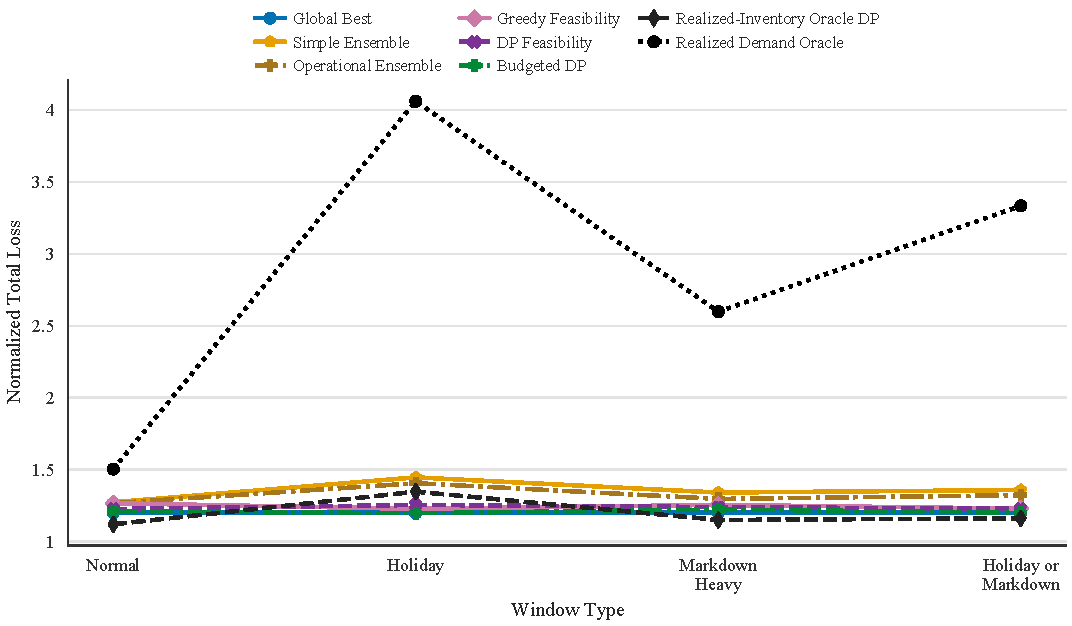
\includegraphics[width=0.85\linewidth]{figures/walmart_window_type_normalized_loss.pdf}
\caption{Walmart normalized planning loss by holiday and markdown stress window.}
\label{fig:walmart-window-normalized-loss}
\end{figure}

\begin{figure}[htbp]
\centering
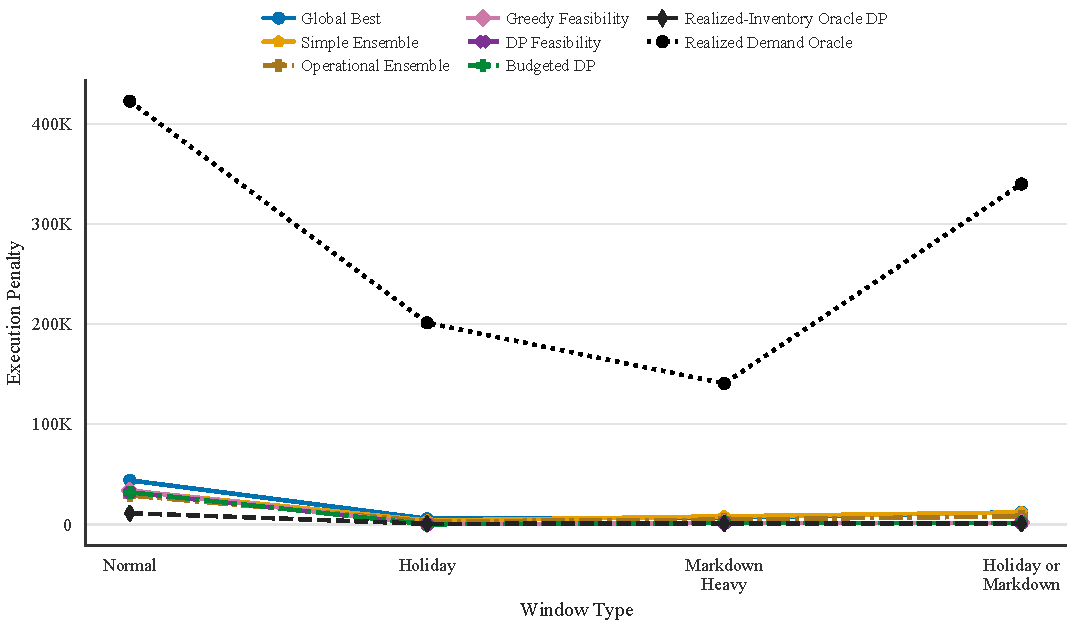
\includegraphics[width=0.85\linewidth]{figures/walmart_window_type_execution_penalty.pdf}
\caption{Walmart execution penalty by holiday and markdown stress window.}
\label{fig:walmart-window-execution-penalty}
\end{figure}

\begin{figure}[htbp]
\centering
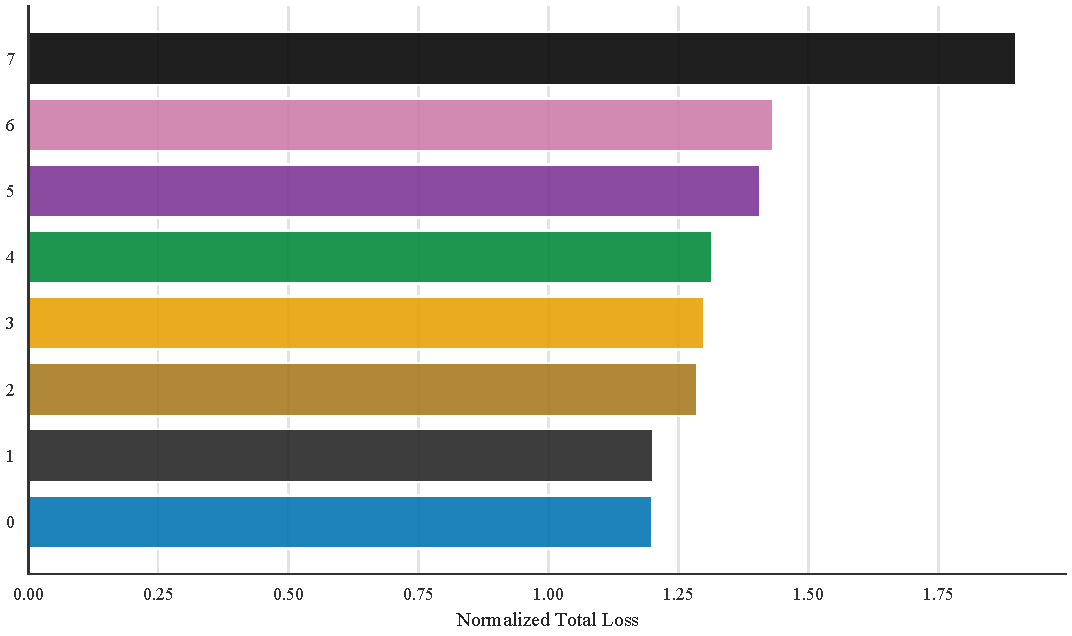
\includegraphics[width=0.85\linewidth]{figures/walmart_weekly_cadence_constraints.pdf}
\caption{Walmart weekly cadence constraint comparison.}
\label{fig:walmart-weekly-cadence}
\end{figure}

\begin{figure}[htbp]
\centering
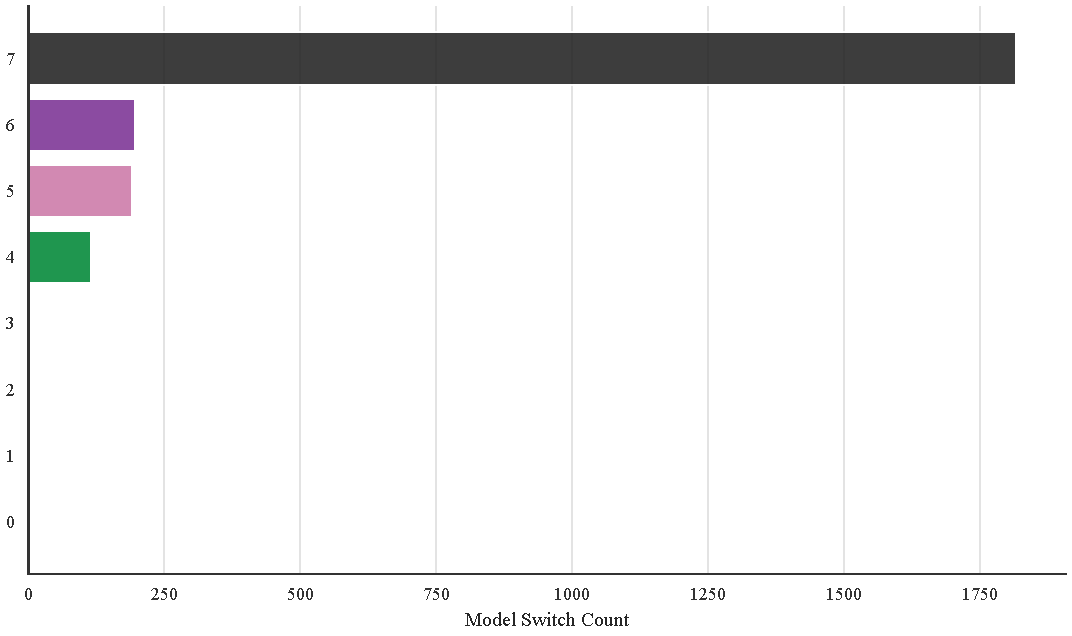
\includegraphics[width=0.85\linewidth]{figures/walmart_budgeted_dp_switching_behavior.pdf}
\caption{Walmart Budgeted-DP switching behavior under weekly cadence constraints.}
\label{fig:walmart-budgeted-dp-switching}
\end{figure}

\section{Citation Completion Notes}

The current draft includes an initial verified reference set for forecasting metrics, retail forecasting benchmarks, inventory control, forecast combination, rolling-horizon decision making, supply-chain planning, and tree-based forecasting models. A later literature pass should still expand coverage of planning nervousness, enterprise planning-system implementation, and execution-risk measurement before submission.
